\documentclass[10pt]{siamltex}
% siamltex     final
\usepackage[]{amsmath,amssymb,epsfig}
%\usepackage[]{graphicx,epsf,epsfig,amsmath,amssymb,amsfonts,latexsym,amsthm}
% \usepackage{bbm}
%\usepackage{amsfonts}
%\usepackage{amsthm}
%% \usepackage[a4paper]{geometry}
%% \geometry{top=0.99in, bottom=0.995in, left=0.995in, right=0.995in}
% \usepackage[top=20mm, bottom=18mm, left=15mm, right=18mm]{geometry}
\usepackage[top=18mm, bottom=18mm, left=20mm, right=20mm]{geometry}

\usepackage{dsfont}
\usepackage{hyperref}

% \graphicspath{{/Users/Mihai/Google Drive/MATLAB/Ranking_Sync/PLOTS/}}
% D:/LATEX/Reports@IIT/figures/
\usepackage{graphicx}
\usepackage[space]{grffile}

\newcommand{\mb}[1]{\mbox{\boldmath$#1$}}

\usepackage{lineno}
\pagewiselinenumbers
\usepackage{graphicx}
\usepackage{amsmath}
\usepackage{amssymb}
\usepackage{graphicx}
\usepackage{comment}
\usepackage{array}
\usepackage{algorithm}
\usepackage{algorithmic}
\usepackage{url}
\usepackage[FIGTOPCAP]{subfigure}
% \usepackage{color}

% \usepackage[toc,page]{appendix}

%\usepackage[outer]{showlabels,rotating}
%\renewcommand{\showlabelsetlabel}[1]
%{\begin{turn}{0}\showlabelfont #1\end{turn}}
%\showlabels{cite}
%\showlabels{ref}
%\showlabels{foo}
%\renewcommand{\showlabelfont}{\small}
\newtheorem{mydef}{Definition}
\newtheorem{mylem}{Lemma}
\usepackage{setspace}
\usepackage{multicol}
\usepackage{multirow}
\usepackage{color}
\usepackage{colortbl}
\usepackage{xcolor}
\usepackage{hyperref}
%\def\Acronimo{ANALYSISOFNETWORKS}
% number the lines

\newcommand{\myreferences}{../../../Postdocs_laptop/postdoc_bib_file}
% \newcommand{\myreferences}{/Users/Mihai/test_bib_file}

\usepackage{lineno}
% \pagewiselinenumbers
%\setlength\linenumbersep{8pt}

% ANALYSISOFNETWORKS
% AALGN
\hypersetup{
%    pdftitle={\Acronimo{}, FP7-PEOPLE-IIF-2012},    % title
%    pdfauthor={Some Author},
    colorlinks=true,
    citecolor=red,
    linkcolor=blue,
    urlcolor=blue
  }

%\newtheorem{theorem}{Theorem}[section]
%\newtheorem{conjecture}[theorem]{Conjecture}
%\newtheorem{corollary}[theorem]{Corollary}
%\newtheorem{proposition}[theorem]{Proposition}
%\newtheorem{lemma}[theorem]{Lemma}
%\newdef{definition}[theorem]{Definition}
%\newdef{remark}[theorem]{Remark}
\newcounter{ale}
\newcommand{\abc}{\item[\alph{ale})]\stepcounter{ale}}
\newenvironment{liste}{\begin{itemize}}{\end{itemize}}
\newcommand{\aliste}{\begin{liste} \setcounter{ale}{1}}
\newcommand{\zliste}{\end{liste}}
\newenvironment{abcliste}{\aliste}{\zliste}

% \usepackage[english]{datetime}



\begin{document}


\begin{pagewiselinenumbers}
\title{Centrality Measure Based on Clusterings in the Effective Resistance Embedding Space}
\author{Kevin Bui\footnotemark[1], Joe Feng\footnotemark[1], Alto Senda\footnotemark[1], Justin Wang\footnotemark[1]  }
\date{ \today}
% \vspace{-10mm}
\maketitle
%\renewcommand{\thefootnote}{\fnsymbol{footnote}}
\footnotetext[1]{Department of Mathematics, UCLA, 520 Portola Plaza, Mathematical Sciences Building 6363, Los Angeles, CA 90095-1555, email: xyz@ucla.edu}
\footnotetext[2]{Second Department, UCLA, 520 Portola Plaza, Mathematical Sciences Building 6363, Los Angeles, CA 90095-1555}
%\renewcommand{\thefootnote}{\arabic{footnote}}

\begin{center}
     February 28, 2015
%  DRAFT
\end{center}

% We propose novel approach to the
\vspace{5mm}

\begin{abstract}
Centrality measures are useful tools in network analysis since they quantify a node's importance in a graph modeling a network. The definition of importance varies based on context, so choosing an appropriate centrality measure is essential. For larger networks in particular, we need to be able to find the most important nodes among hundreds or thousands of them. We propose a new centrality measure called $k$-means centrality based on applying $k$-means to the effective resistance embedding. The effective resistance embedding is derived from using Spielman-Srivastava's algorithm \cite{Spielman2011} in order to compute the effective resistance of a graph when representing it as an electrical network. $k$-means centrality measures the connectedness of one node to all other clusters on the graph computed by $k$-means. This measure has potential use in social network analysis since it determines the number of communities a node is a part of within a graph. We compare the results of our new measure to those of the already established betweenness and closeness centrality measures and their current-flow variants. Numerical results show that $k$-means centrality produces results similar to other centrality measures. However, they show that it is not the most discriminative measure, but it has the highest correlation with the degrees of the nodes. 
\end{abstract}


\begin{keywords} network-means centrality, electrical network, $k$-means, spectral graph theory
\end{keywords}


\section{Introduction}

The concept of centrality is investigated in order to answer the question, "What is the most important nodes in a network?" Centrality is an important measure used in social, biological, communication, and transportation networks since it helps analyze the relative structural prominence of nodes in the network. Especially in social network analysis it can measure the most influential or the most connected person depending on the context of the network. Two most frequently utilized centrality measures in this area are betweenness centrality and closeness centrality since they both account for the information that travels on the shortest paths of the network. However, since both centrality measures ignore information spread along non-shortest paths, current-flow betweenness centrality and current-flow closeness centrality were proposed by Brandes and Fleischer \cite{brandes2005centrality} to account for that. These variants are based on representing a graph as an electrical network where electrical current is propagated throughout the whole network.

In this paper, we review betweenness, closeness, and their current-flow variants and we also propose a new centrality measure called $k$-means centrality which is based on applying the  $k$-means algorithm to the effective resistance embedding. The effective resistance embedding is a higher dimensional embedding of the nodes derived from computing the effective resistance of a graph representing an electrical network. Finally, we present numerical results comparing the proposed centrality measure to the aforementioned measures. 

\section{Centrality Measures}
Throughout the paper, we consider only the graphs $G = (V,E)$ that are simple, undirected, and connected and that have $n \geq 3$ nodes. 
\subsection{Centrality Measures Based on Shortest Paths}
Based on information travelling on shortest paths of a network, betweenness centrality and closenness centrality are the most popular yet most basic measures used in network analysis. 

Betweenness centrality \cite{booknewman, brandes2005centrality} $c_B: V \rightarrow \mathbb{R}_{\geq 0}$ measures the extent to which a node lies on the shortest paths between other nodes. It is defined as 
\begin{align}
c_B(v) = \frac{1}{n_B} \sum_{s,t \in V} \frac{\sigma_{st}(v)}{\sigma_{s,t}},
\end{align}
where $\sigma_{st}(v)$ is the number of shortest paths from $s$ to $t$ containing $v$ as an inner vertex, $\sigma_{s,t}$ is number of shortest paths from $s$ to $t$, and $n_B = (n-1)(n-2)$ is a normalizing constant.



On the other hand, closeness centrality $c_C: V \rightarrow \mathbb{R}$ \cite{booknewman, brandes2005centrality} measures the mean distance from a node to other nodes. It is defined as 
\begin{align}
c_{C}(v)=\frac{n_{C}}{\sum\limits_{t\neq v} d_{G}(v,t)}
\end{align}
where $n_C = n-1$ is a normalizing constant and
$d_{G}(v,t)$ denotes the length of the shortest path between $v$ and $t$.
     
     Measures based on shortest paths do not account for the spread of information along non-shortest paths. Consequently, they are a poor metric for systems in which information flow behaves this way. Resolving this issue, current-flow betweenness centrality and current-flow closeness centrality account for the spread of information along non-shortest paths. Before we review their definitions, we will discuss how a graph can be represented as an electrical network.
     %Edited: Consequently, it may be difficult to distinguish between nodes with high centrality measures and those with low centrality measures. ->  Consequently, they are a poor metric for systems in which information flow behaves this way.
     \subsection{Graph as an Electrical Network \cite{brandes2005centrality}} A graph can be represented as an electrical network $N = (G;c)$ with positive edge weights $c: E \rightarrow \mathbb{R}_{> 0}$ indicating the conductance of an edge. Since we are dealing with undirected graphs in this paper, we have $c(e) = 1$.
     
     To represent how current flows throughout an electrical network, a vector $b: V \rightarrow \mathbb{R}$ called supply defines where current externally enters and leaves it. A node $v \in V$ is a source if $b(v) > 0$ and is a sink if $b(V) < 0$. By conservation, $\sum_{v \in V} b(v) = 0$ is required. For simplicity, we only consider the unit current entering the network with a single source and a single sink, so 
        \begin{align*}
     b_{st}(v) =
\begin{cases}
1, & \text{if }v=s 
\\
-1, & \text{if }v=t
\\
0 & \text{otherwise}
\end{cases}
     \end{align*}

To account for the direction of the current, each edge is given an arbitrary orientation. Furthermore, we denote $\vec{e}$ as the directed edge corresponding to the orientation of $e \in E$ and $\vec{E}$ as the set of all oriented edges. Now we will define $x: \vec{E} \rightarrow \mathbb{R}$ as the current of the graph and introduce a lemma relating to it. 
\vspace{5mm}
\begin{mydef}
Let $N = (G;c)$ be an electrical network with supply $b$. A vector $x: \vec{e} \rightarrow \mathbb{R}$ is called a \emph{current} if it satisfies the following:
\begin{enumerate}
\item Kirchoff's Current Law
\begin{align}
\sum_{(v,w) \in \vec{E}} x(v,w) - \sum_{(u,v) \in \vec{E}} x(u,v) = b(v) \quad \textrm{for all} \quad v \in V
\end{align}
\item Kirchoff's Potential Law
\begin{align}
\sum_{i=1}^k x(\vec{e_i}) = 0 \quad \textrm{for every cycle} \quad e_1, ..., e_k \quad \textrm{in} \quad G.
\end{align}
\end{enumerate}
\end{mydef}

\begin{mylem}
For an electrical network $N = (G;c)$ and any supply $b$, there is a unique current $x: \vec{E} \rightarrow \mathbb{R}$.
\end{mylem}
\vspace{5mm}

A value $x(\vec{e}) > 0$ indicates that the current is flowing in the direction of $\vec{e}$; $x(\vec{e}) < 0$ indicates that the current is flowing against the direction of $\vec{e}$. For an $st$-supply, we denote $x_{st}$ as the $st$-current. Furthermore, current is related to potential difference $\hat{p}: \vec{E} \rightarrow \mathbb{R}$ such that $\hat{p}(\vec{e}) = x(\vec{e})/c(e)$ for all $e \in E$. A vector $p: V \rightarrow \mathbb{R}$ assigns absolute potentials if $\hat{p}(v,w) = p(v) - p(w)$ for all $(v,w) \in \vec{E}$. We use $\hat{p}_{st}$ and $p_{st}$ to indicate that the potential differences and the absolute potentials respectively are based on the $st$-supply.
\vspace{5mm}
\begin{mylem}
Let $N = (G;c)$ be an electrical network with supply b. For any fixed vertex $v_1 \in V$ and constant $p_1 \in \mathbb{R}$, there are unique absolute potentials $p: V \rightarrow \mathbb{R}$ with $p(v_1) = p_1$.
\end{mylem}
\vspace{5mm}
\begin{mylem}
The absolute potentials of an electrical network $N = (G;c)$ with supply $b$ are exactly the solutions of $Lp=b$ where $L$ is the Laplacian matrix defined as follows:
\begin{align}
     L(v,w)=
\begin{cases}
\sum_{e: v \in e} c(e), & \text{if }v=w 
\\
-c(e), & \text{if }e={v,w}
\\
0 & \text{otherwise}
\end{cases}
\end{align}
for all $v,w \in V$.
\end{mylem}
\vspace{5mm}

Lemma 3 shows that computing the absolute potentials of an electrical network is possible, but since $L$ is singular, there are multiple assignments of absolute potentials for a given supply $b$. However, by Lemma 2, we can set $p(v_1) = 0$ to solve for only one assignment given the fixed vertex ordering $v_1, v_2, ..., v_n$. To do so, we omit the row and column corresponding to $v_1$ in $L$ to obtain $\widetilde{L} \in \mathbb{R}^{n-1 \times n-1}$. Since $\widetilde{L}$ is positive definite and regular, we obtain
\begin{align}
\label{lp_equation}
     p = \left( \begin{array}{cc}
0 & \mathbf{0}^T \\
\mathbf{0} & \widetilde{L}^{-1} \\
\end{array} \right) b
     \end{align}
     \vspace{5mm}
     With all the necessary theory established, we now review the current-flow variants of betweenness and closeness.
     \subsection{Current-Flow Betweenness Centrality}
     The amount of $st$-current flowing through a node is the analog of the number of shortest paths passing through it for betweenness centrality. Given a supply $b$ and the $st$-current, we define throughput of a vertex $v \in V$ as
     \begin{align}
     \tau_{st}(v) = \frac{1}{2}\left( -\left|b(v) \right| + \sum_{e: v \in e} \left|x(\vec{e})\right|\right)
     \end{align}
     to represent the amount of current flowing through $v$. The throughput is well-defined because of Lemma 1, where $x$ is unique for a given supply $b$.
     
     Current-flow betweenness centrality $c_{CB}(v): V \rightarrow \mathbb{R}_{\geq 0}$ is defined as 
     \begin{align}
     c_{CB}(v) = \frac{1}{n_B} \sum_{s,t \in V} \tau_{st}(v) \quad \textrm{for all} \quad v \in V
     \end{align}
     where $n_B = (n-1)(n-2)$\cite{brandes2005centrality}. Because calculating throughput for current-flow betweenness is computationally difficult, we use a randomized approximation algorithm summarized below to approximate the centrality measure. 
\begin{algorithm}                      % enter the algorithm environment
\caption{Randomized approximation scheme for current-flow betweenness \cite{brandes2005centrality}}          % give the algorithm a caption
\label{alg1}                           % and a label for \ref{} commands later in the document
\begin{algorithmic}                    % enter the algorithmic environment
    \REQUIRE electrical network $N = (G; c)$, threshold $\epsilon > 0$, constant $l$
\RETURN current-flow betweenness approximation $c'_{CB}: V \rightarrow \mathbb{R}_{\geq 0}$
   \STATE $c'_{CB} \leftarrow \mathbf{0}$ and $k \leftarrow l \cdot \lceil (c^*/\epsilon)^2 \textrm{log } n \rceil$ where $c^* = n(n-1)/n_B$.
   \FOR{$i=1,...,k$}
   \STATE select $s \neq t \in V$ uniformly at random and solve $Lp = b_{st}$ according to Equation \ref{lp_equation}
   \FOR{$v \in V \setminus \{s,t\}$}
   \FOR{$e \in \{v,w\} \in E$}
   \STATE increase $c'_{CB}(v) by c(e) \cdot \left| \widetilde{p}(v) - \widetilde{p}(w) \right| \cdot c^*/2k$
   \ENDFOR
   \ENDFOR
   \ENDFOR
\end{algorithmic}
\end{algorithm}
\subsection{Current-Flow Closeness Centrality}
Current-flow closeness centrality $c_{CC}: V \rightarrow \mathbb{R}_{>0}$ is defined by 
\begin{align}
c_{CC}(s) = \frac{n_C}{\sum_{t \neq s} p_{st}(s) - p_{st}(t)} \quad \textrm{for all} \quad s \in V \quad \cite{brandes2005centrality}.
\end{align}
Current-flow centrality is well-defined by Lemma 2 since any two absolute potentials differ only by an additive constant. The term $p_{st}(s) - p_{st}(t)$ is an alternative measure of distance between $s$ and $t$ given the unit $st$-current, making it a current-flow variant of closeness centrality.

To compute the effective resistance between any two nodes, we use Spielman-Srivastava's algorithm summarized below. Since the solution $X$ is a $n \times O(\textrm{log } n)$ matrix, each row can be interpreted as an embedding of the corresponding vertex to the $O(\textrm{log }n)$-dimensional Euclidean space. We call $X$ the effective resistance embedding. Because the effective resistance embedding is higher dimensional, we may apply the $k$-means algorithm to obtain graph clusters. This motivates us to propose a new centrality measure.

\begin{algorithm}                    % enter the algorithm environment
\caption{Approximating Effective Resistances \cite{Spielman2011}}          % give the algorithm a caption
\label{alg2}                           % and a label for \ref{} commands later in the document
\begin{algorithmic}                    % enter the algorithmic environment
    \REQUIRE Laplacian matrix $L$, incident matrix $B$, random Johnson-Lindenstrauss projection of size $m \times O(\textrm{log } n)$
\RETURN effective resistance between nodes $i$ and $j$ 
\STATE Solve the system $LX = B^{T}Q$
\STATE Compute $\|X_i - X_j\|_2$ where $X_i$ is the $i$th-row of $X$ for effective resistance $p_{st}(i) - p_{st}(j)$
\end{algorithmic}
\end{algorithm}
\subsection{$k$-Means Centrality}
By applying the $k$-means algorithm to the effective resistance embedding, we obtain a partitioning of the nodes into $k$ sets: $\{S_1, S_2, ..., S_k\}$. Based on the results, we define a new centrality measure called $k$-means centrality. We define $k$-means centrality $c_K(s): V \rightarrow \mathbb{R}_{\geq 0}$ as 
\begin{align}
c_K(s) = \sum_{k=2}^L \sum_{t \neq s} \mathbf{1}_{\{ \textrm{edge } st \textrm{ is a cut edge in } \{S_1^{(k)}, S_2^{(k)}, ..., S_k^{(k)}\}\} } \quad \textrm{for all} \quad s \in V.
\end{align}
where a cut edge is an edge whose nodes are part of two different partition sets and $\mathbf{1}$ is the indicator function. This centrality measure computes the propensity of a node to lie on a cut edge when partitioning the graph into $k$ clusters for different values of $k$ ranging from $2$ to some constant $L$. 


\section{Numerical Experiments}  \label{sec:NumExpSyn}
In this section, we compute the centrality measures on two synthetic data and two real data and compare them. We also analyze how discriminative each measure is and how correlated it is to the degrees of the nodes. From our results, we would like to see how effective $k$-means centrality is as a centrality measure compared to the others.

The visual representations of the graphs we produce were created by using Pajek, so nodes with larger centrality have larger size and they are closer to violet on the spectrum. Likewise, nodes with smaller centrality have smaller size and they are closer to red on the spectrum.

%%%%%%%%%%%%%%%%%%%%%%%%%%%%%%%%%%%%%%%%%%%%%%%%
\hfill

\subsection{A Toy Network}
We compute the centrality measures for the graph shown in Figure \ref{fig:ToyGraph}. Because nodes $A$ and $B$ are most central, they are expected to have high centrality values. Furthermore, being a symmetric graph, opposite nodes are expected to have the same centrality values. The results are shown in Figure \ref{fig:centrality1}.

\begin{figure}[ht]
\begin{center}
\includegraphics[width=0.56\columnwidth]{toy1}
\end{center}
\caption{Toy Graph}
\label{fig:ToyGraph}
\end{figure}
As expected, nodes A and B show higher centrality values than the other nodes for all five centrality measures. However, current-flow closeness centrality and $k$-means centrality lack symmetry in their values. The asymmetry for current-flow closeness is attributed to the Spielman-Srivastava's algorithm used to approximate effective resistance. The result shows that the algorithm performs poorly on small networks. As for $k$-means centrality, the random initial assignments of centroids for every run of the $k$-means algorithm may have caused the asymmetry. 
\begin{figure}[ht]
\centering
\subfigure[Betweenness Centrality of Toy Graph]{
    \includegraphics[width=0.45\textwidth]{toy_betweenness}
}
\subfigure[Closeness Centrality of Toy Graph]{
    \includegraphics[width=0.45\textwidth]{toy_closeness}
}
\subfigure[Current-Flow Betweenness Centrality of Toy Graph]{
    \includegraphics[width=0.45\textwidth]{toy_current_flow_betweenness}
}
\subfigure[Current-Flow Closeness Centrality of Toy Graph]{
    \includegraphics[width=0.45\textwidth]{toy_current_flow_closeness}
}
\subfigure[$k$-Means Centrality of Toy Graph]{
    \includegraphics[width=0.45\textwidth]{toy_k_centrality}
}
\caption{Centrality Measures of Toy Graph}
\label{fig:centrality1}
\end{figure}

\subsection{The "Tripartite" Graph}
We compute the centrality measures on what we call the "tripartite" graph, which is shown in Figure \ref{fig:Tripartite Graph}. This graph has three major clusters of nodes: both outer clusters have 100 nodes and the inner cluster has 50 nodes. Within each cluster, nodes are connected to another with high probability, and the nodes of the outer clusters are connected to the nodes of the inner cluster with also a high probability. In addition, there is a small number of edges between the two outer clusters. The results of the "tripartite" graph is shown in Figure \ref{fig:centrality2}.

We observe that betweenness centrality performs exceptionally poorly on this graph because most of the nodes have low centrality values. This result is attributed to the edges between the outer clusters since they form some of the shortest paths of the graph. Moreover, we see that current-flow closeness centrality does not have as many nodes with low centrality values and nodes with high centrality values as the other centrality measures. Most of its nodes have intermediate centrality values instead. All the other centrality measures produce similar results. 

\begin{figure}[h!]
\begin{center}
\includegraphics[width=0.56\columnwidth]{tripartite}
\end{center}
\caption{Tripartite Graph}
\label{fig:Tripartite Graph}
\end{figure}

Because the graph have 250 nodes, we need to perform further tests to better analyze the centrality measures. We perform two tests: cluster recovery and average distance. 

The cluster recovery test attempts to separate the graph based on the centrality measures into two partitions: the partition corresponding to the outer clusters and the partition corresponding to the inner cluster. We run $k$-means on the vector of centrality values with $k=2$, thus producing a vector of indices of values either 1 or 2. The vector of the centrality values are ordered from 100 nodes of the left outer cluster, 50 nodes of the inner cluster, and finally 100 nodes of the right outer cluster. Thus a centrality measure performs well on this test if the first 100 nodes and the last 100 nodes are clustered in one group and the rest in another group. The results for this test are shown in Figure \ref{fig:test1}.

According to our results, the centrality scores of closeness, current-flow betweenness, and $k$-means centrality were successfully partitioned into two representative clusters of the "tripartite" graph. Betweenness clustered majority of the nodes into one group. Current-flow closeness was successful in classifying the middle 50 nodes into one group, but some of the outer nodes, corresponding to the first and last 100 clusters, are clustered in the same group. This shows that current-flow closeness is vulnerable to noise, which are the edges between the outer clusters of the "tripartite" graph.
\begin{figure}[h!!]
\centering
\subfigure[Betweenness Centrality of "Tripartite" Graph]{
    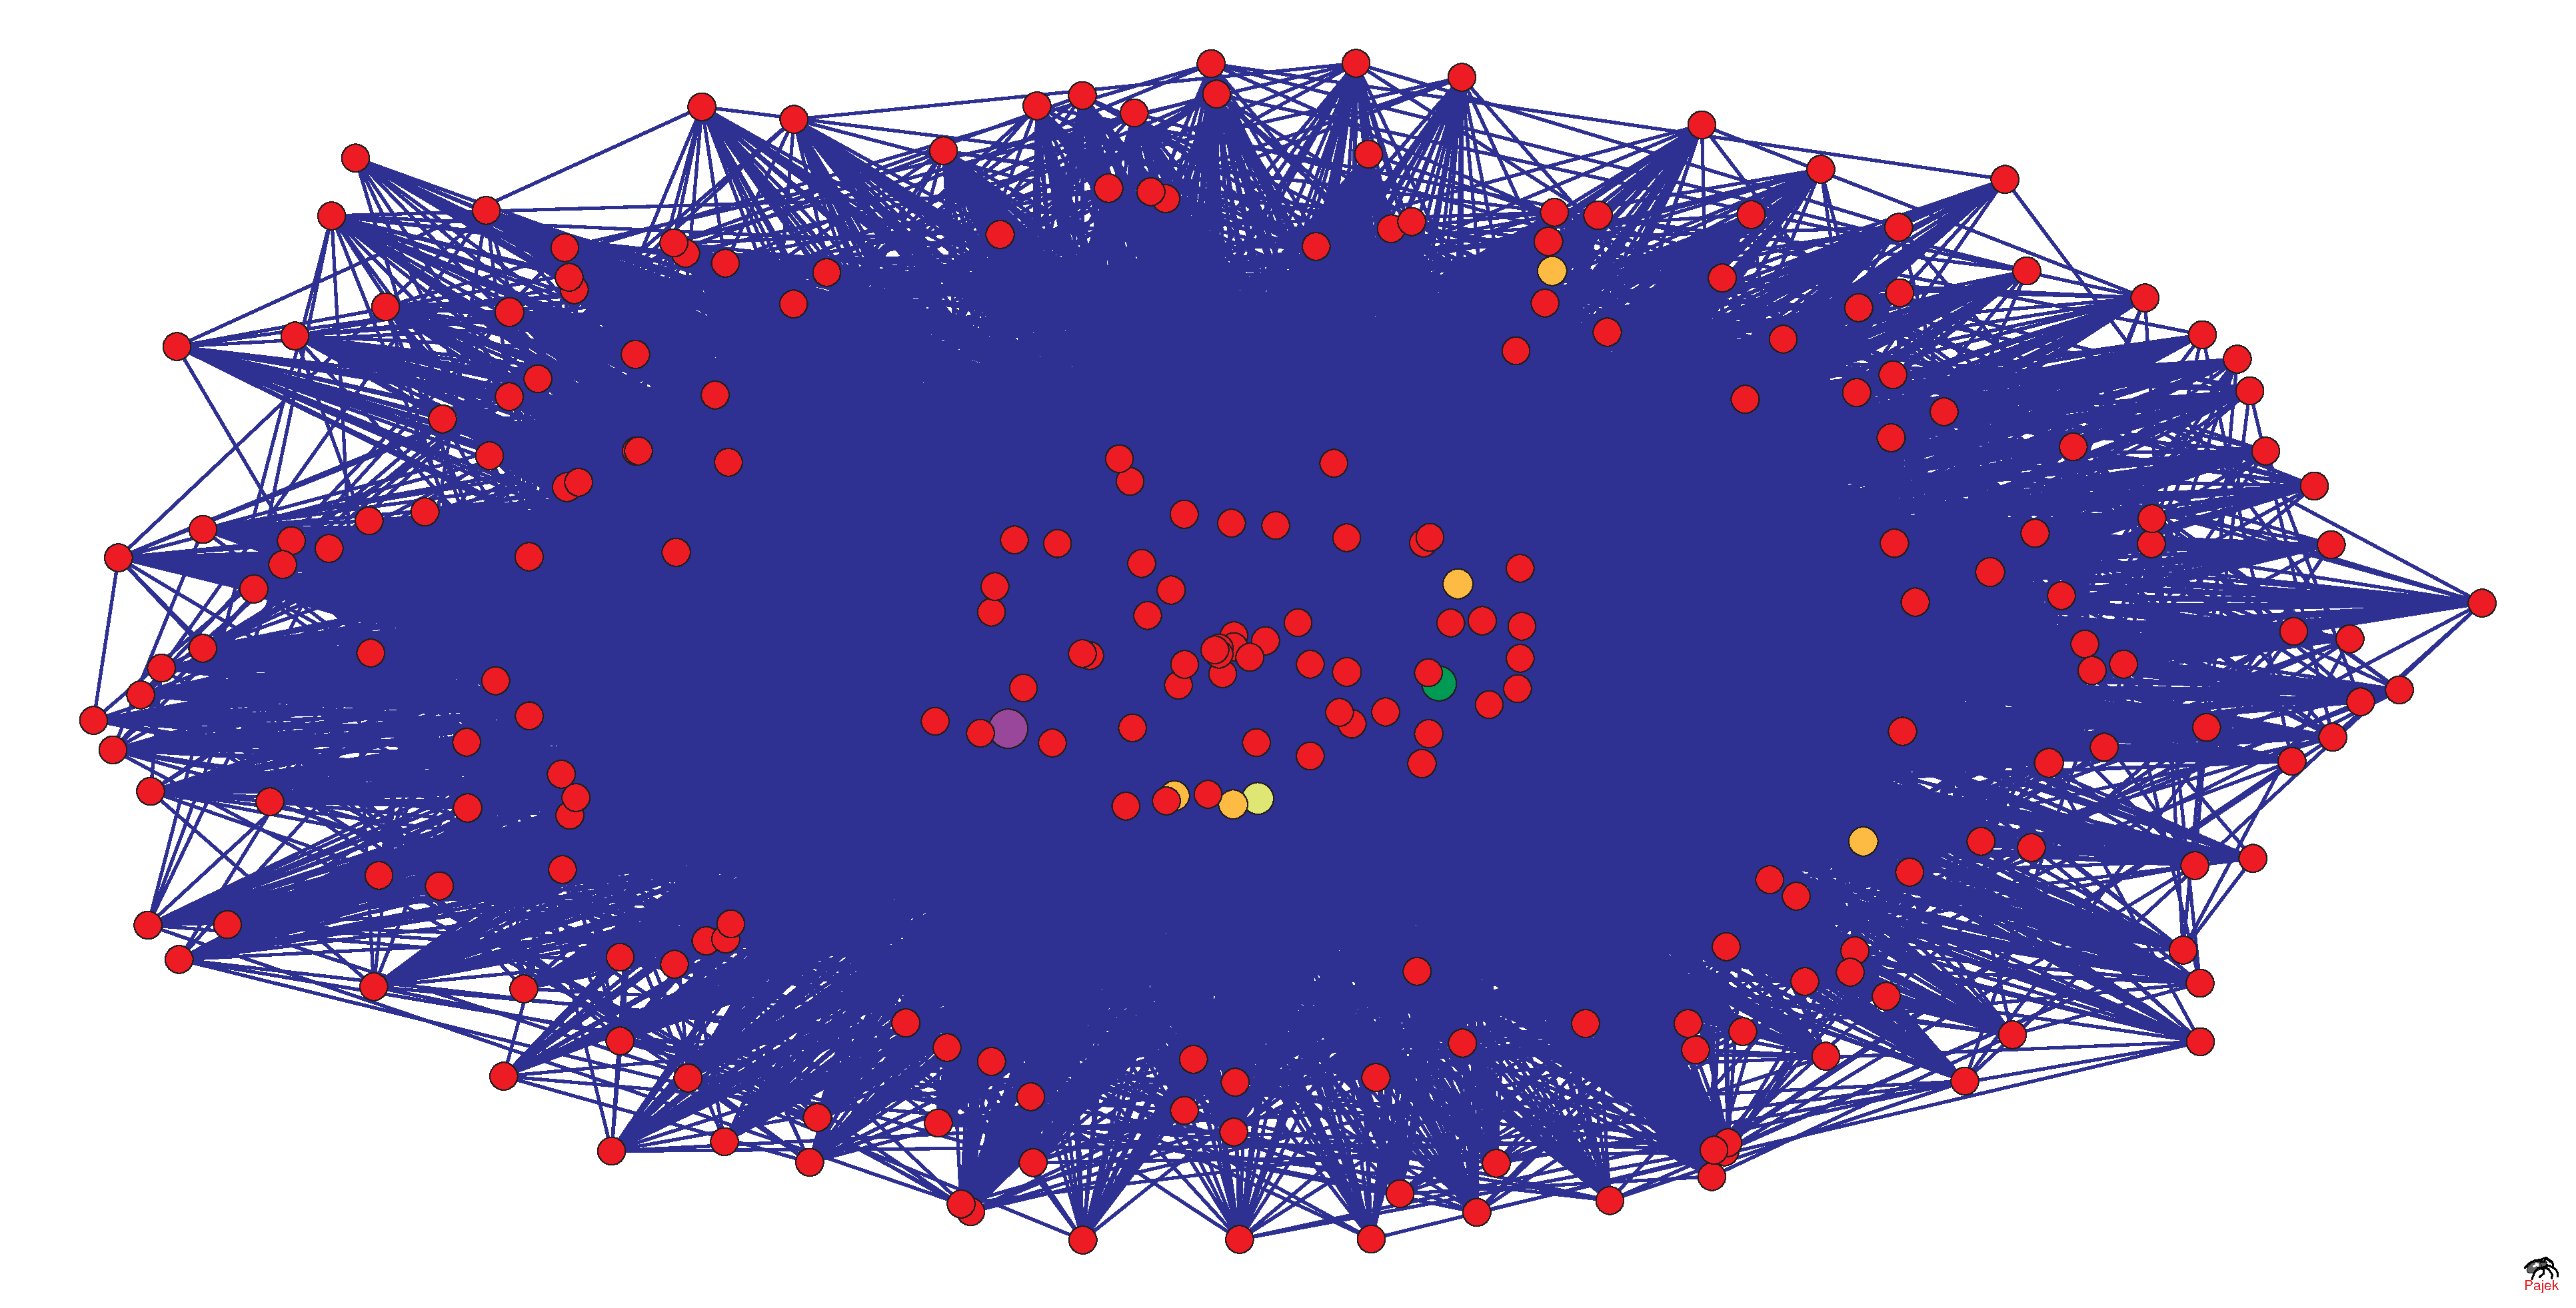
\includegraphics[width=0.45\textwidth]{toy2_betweenness2}
}
\subfigure[Closeness Centrality of "Tripartite" Graph]{
    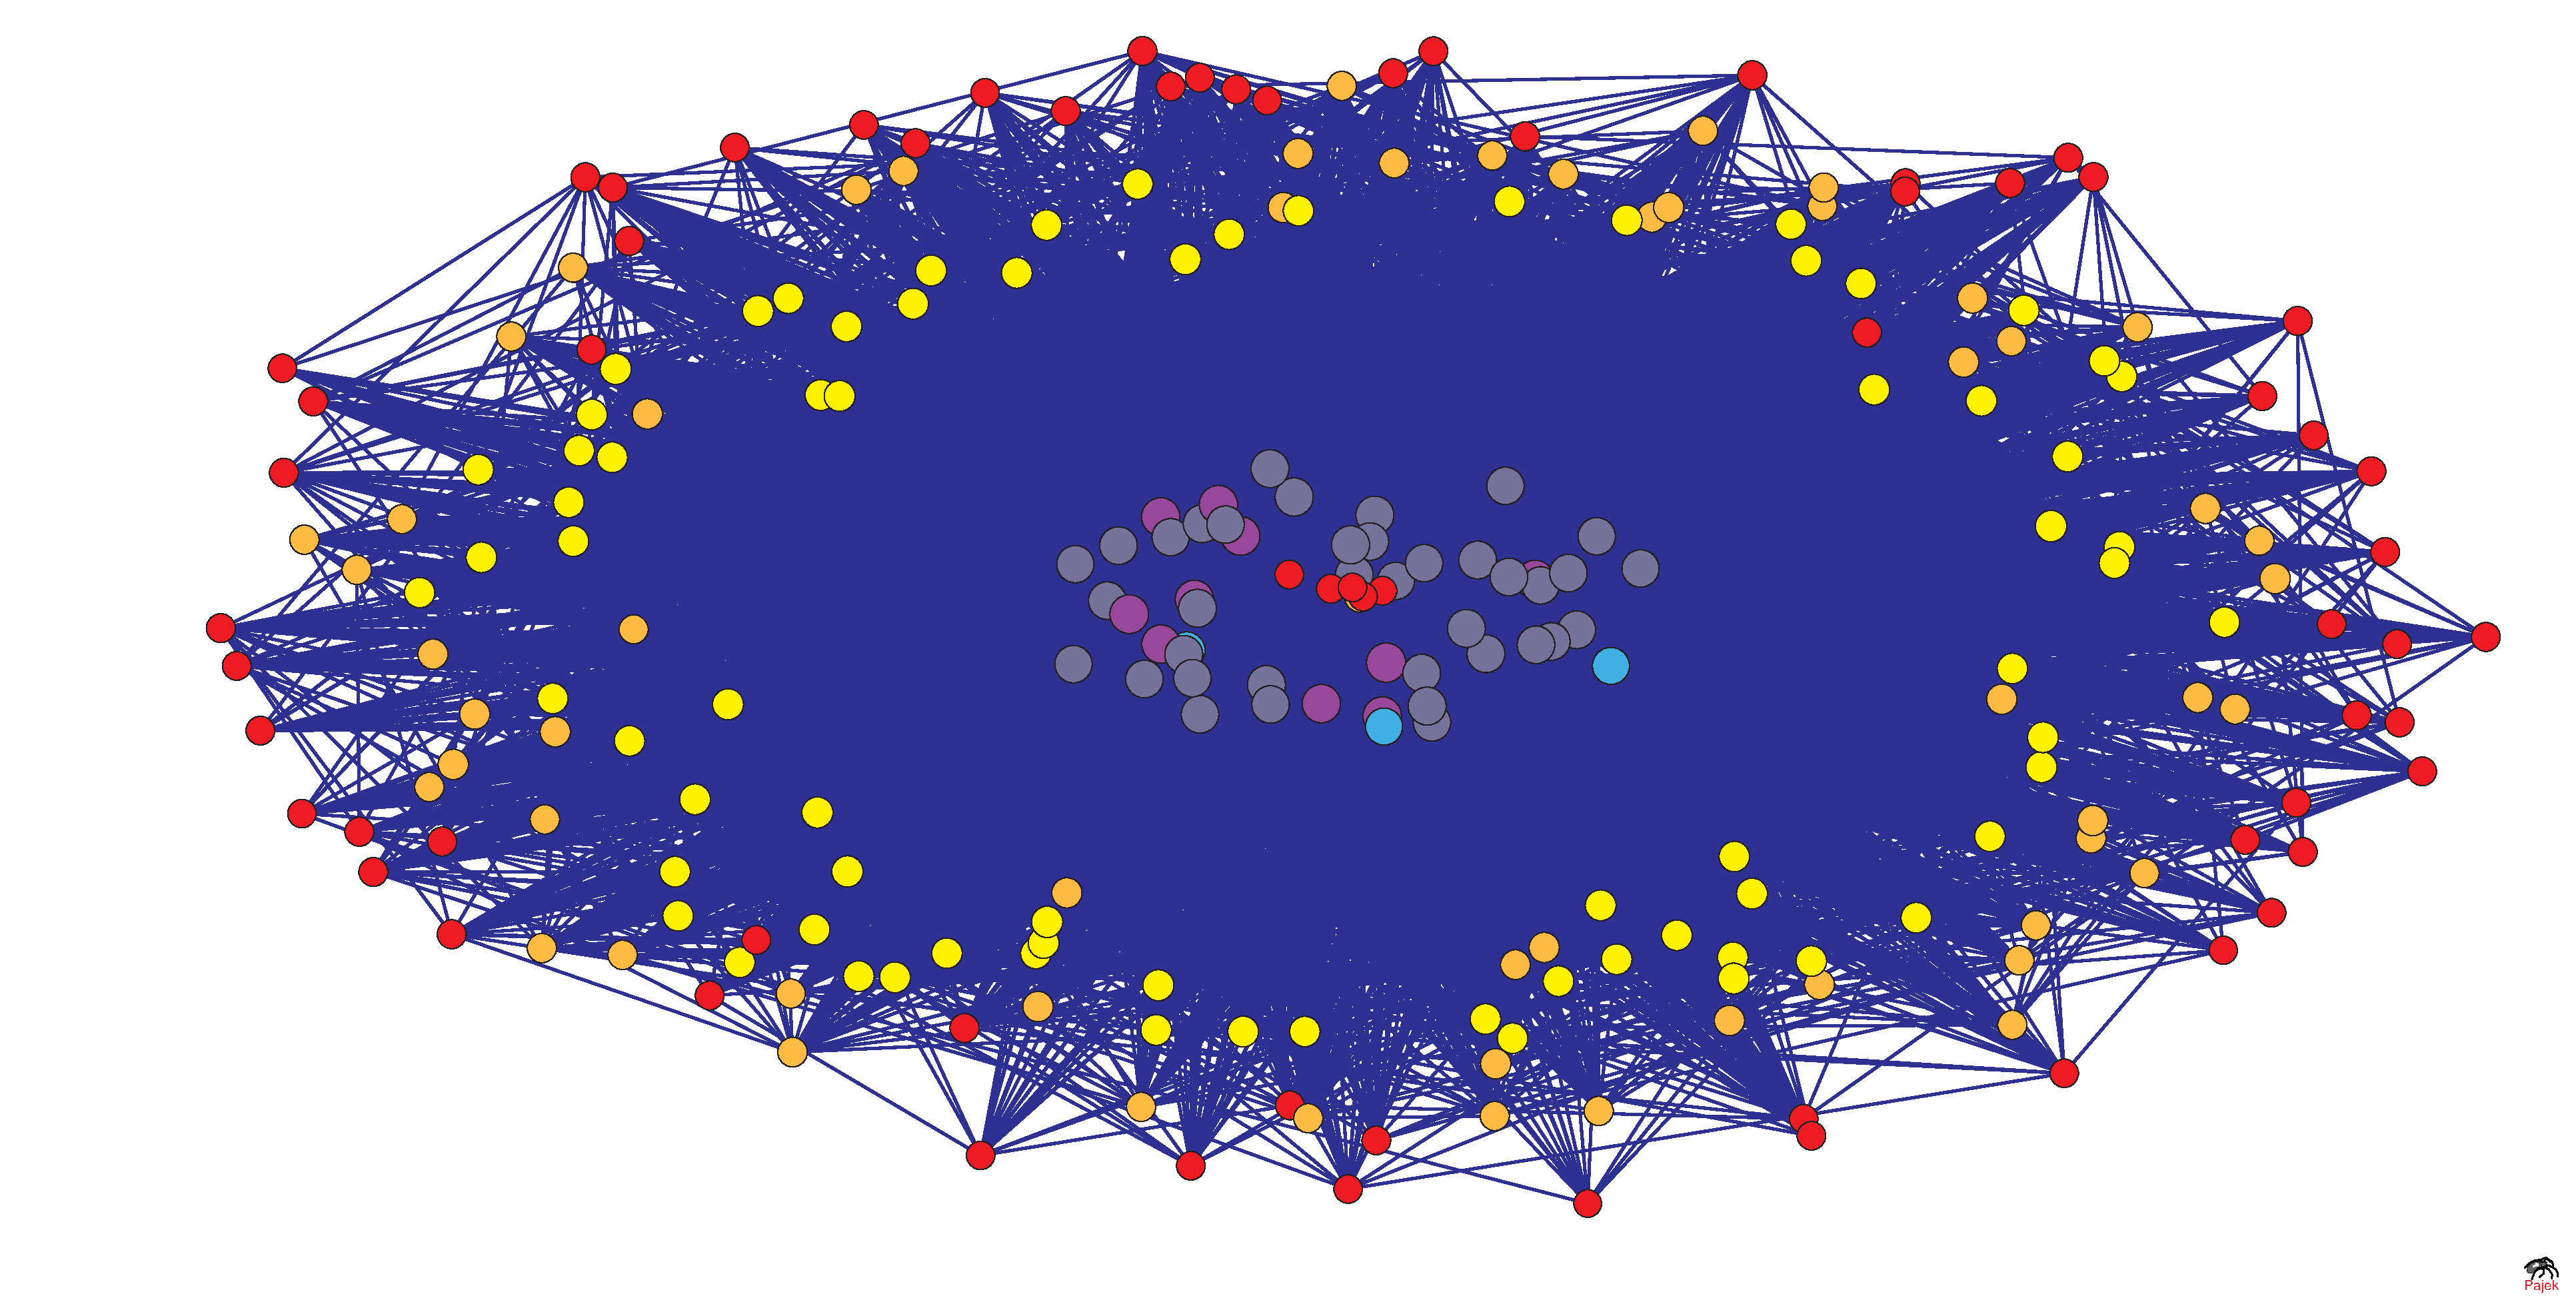
\includegraphics[width=0.45\textwidth]{toy2_closeness2}
}
\subfigure[Current-Flow Betweenness Centrality of "Tripartite" Graph]{
    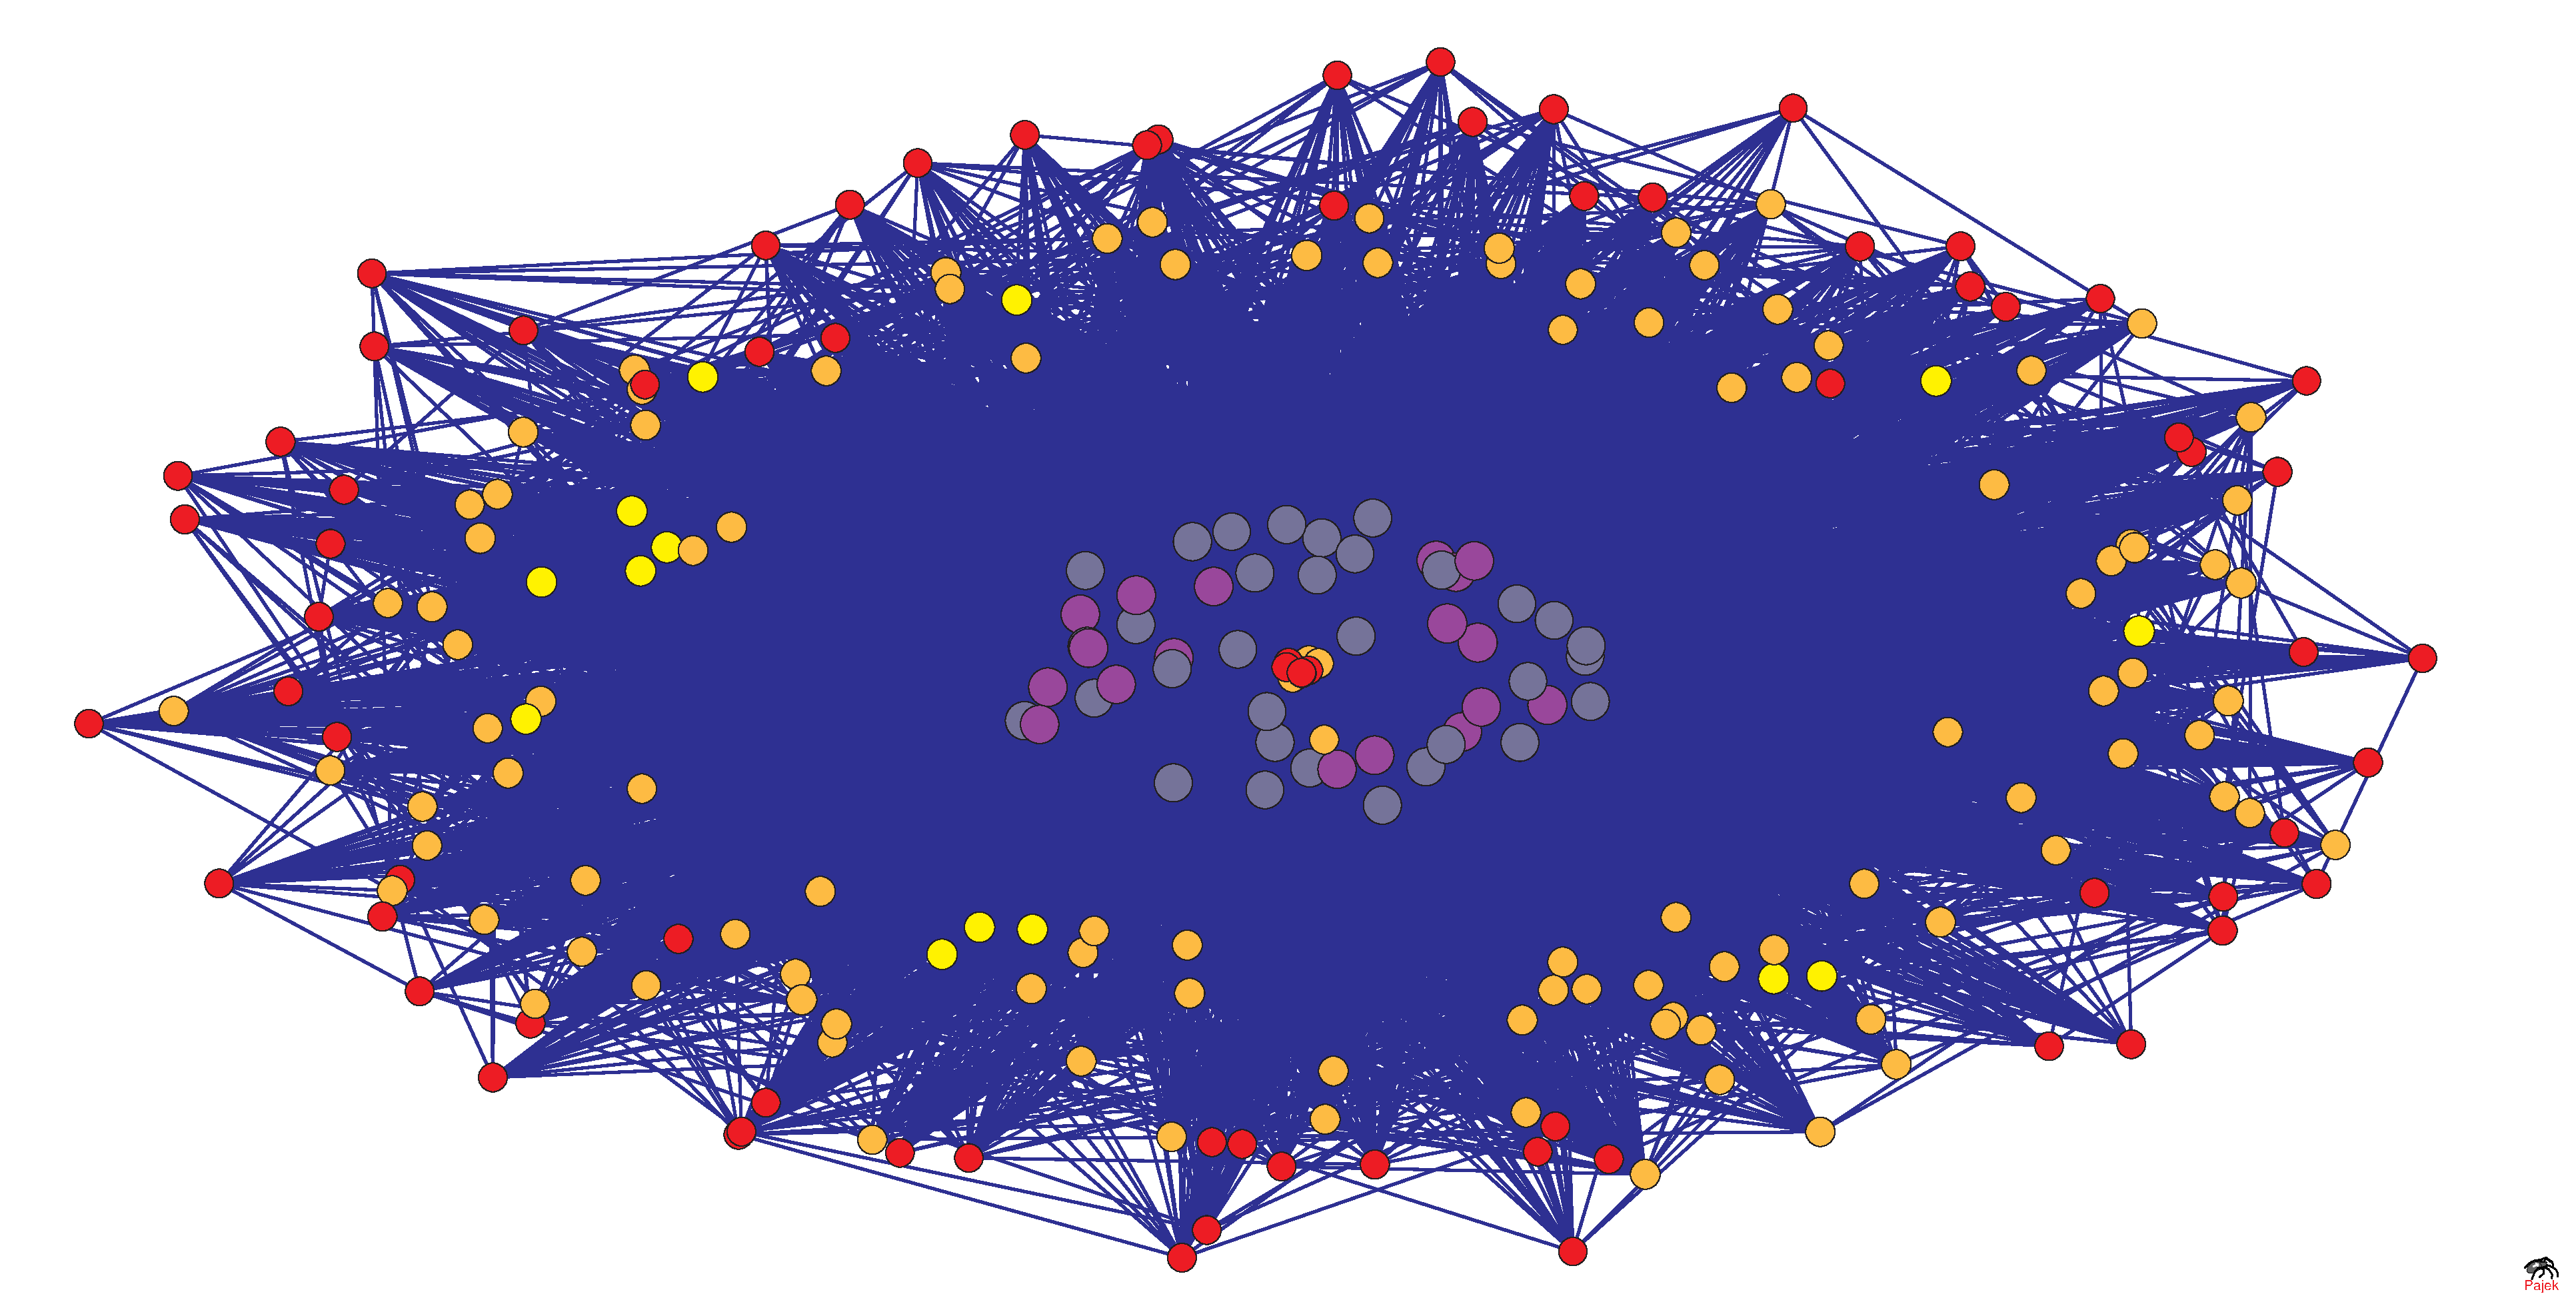
\includegraphics[width=0.45\textwidth]{toy2_current_flow_betweenness}
}
\subfigure[Current-Flow Closeness Centrality of "Tripartite" Graph]{
    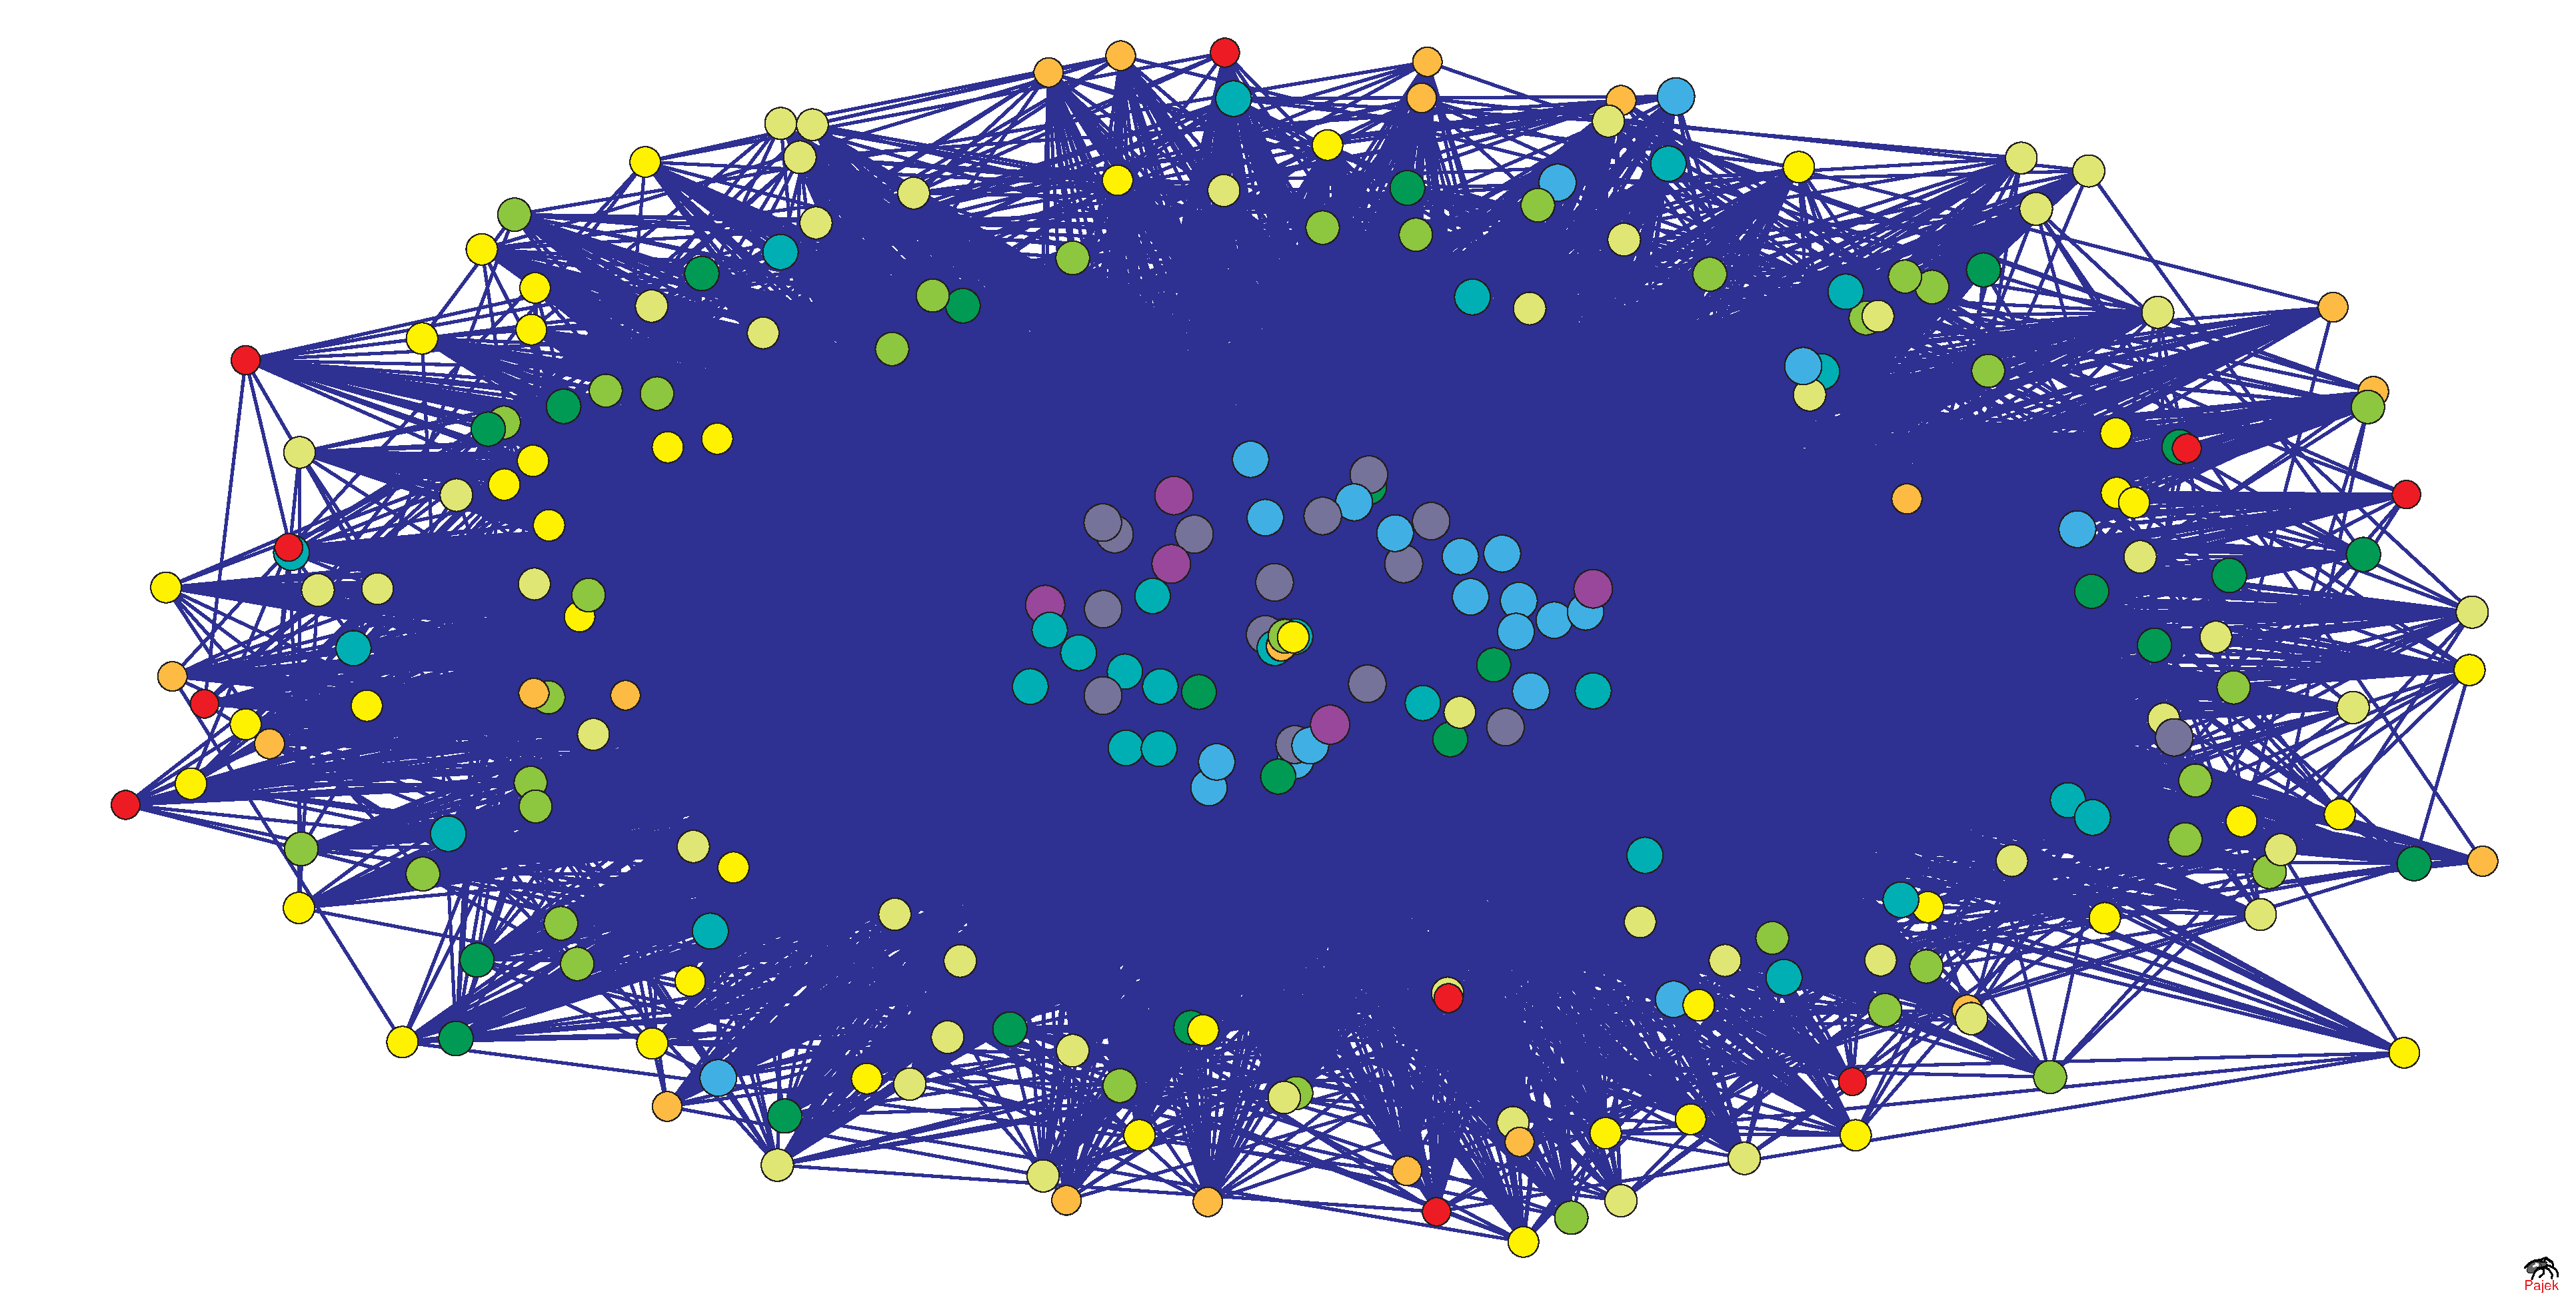
\includegraphics[width=0.45\textwidth]{toy2_current_flow_closeness}
}
\subfigure[$k$-Means Centrality of "Tripartite" Graph]{
    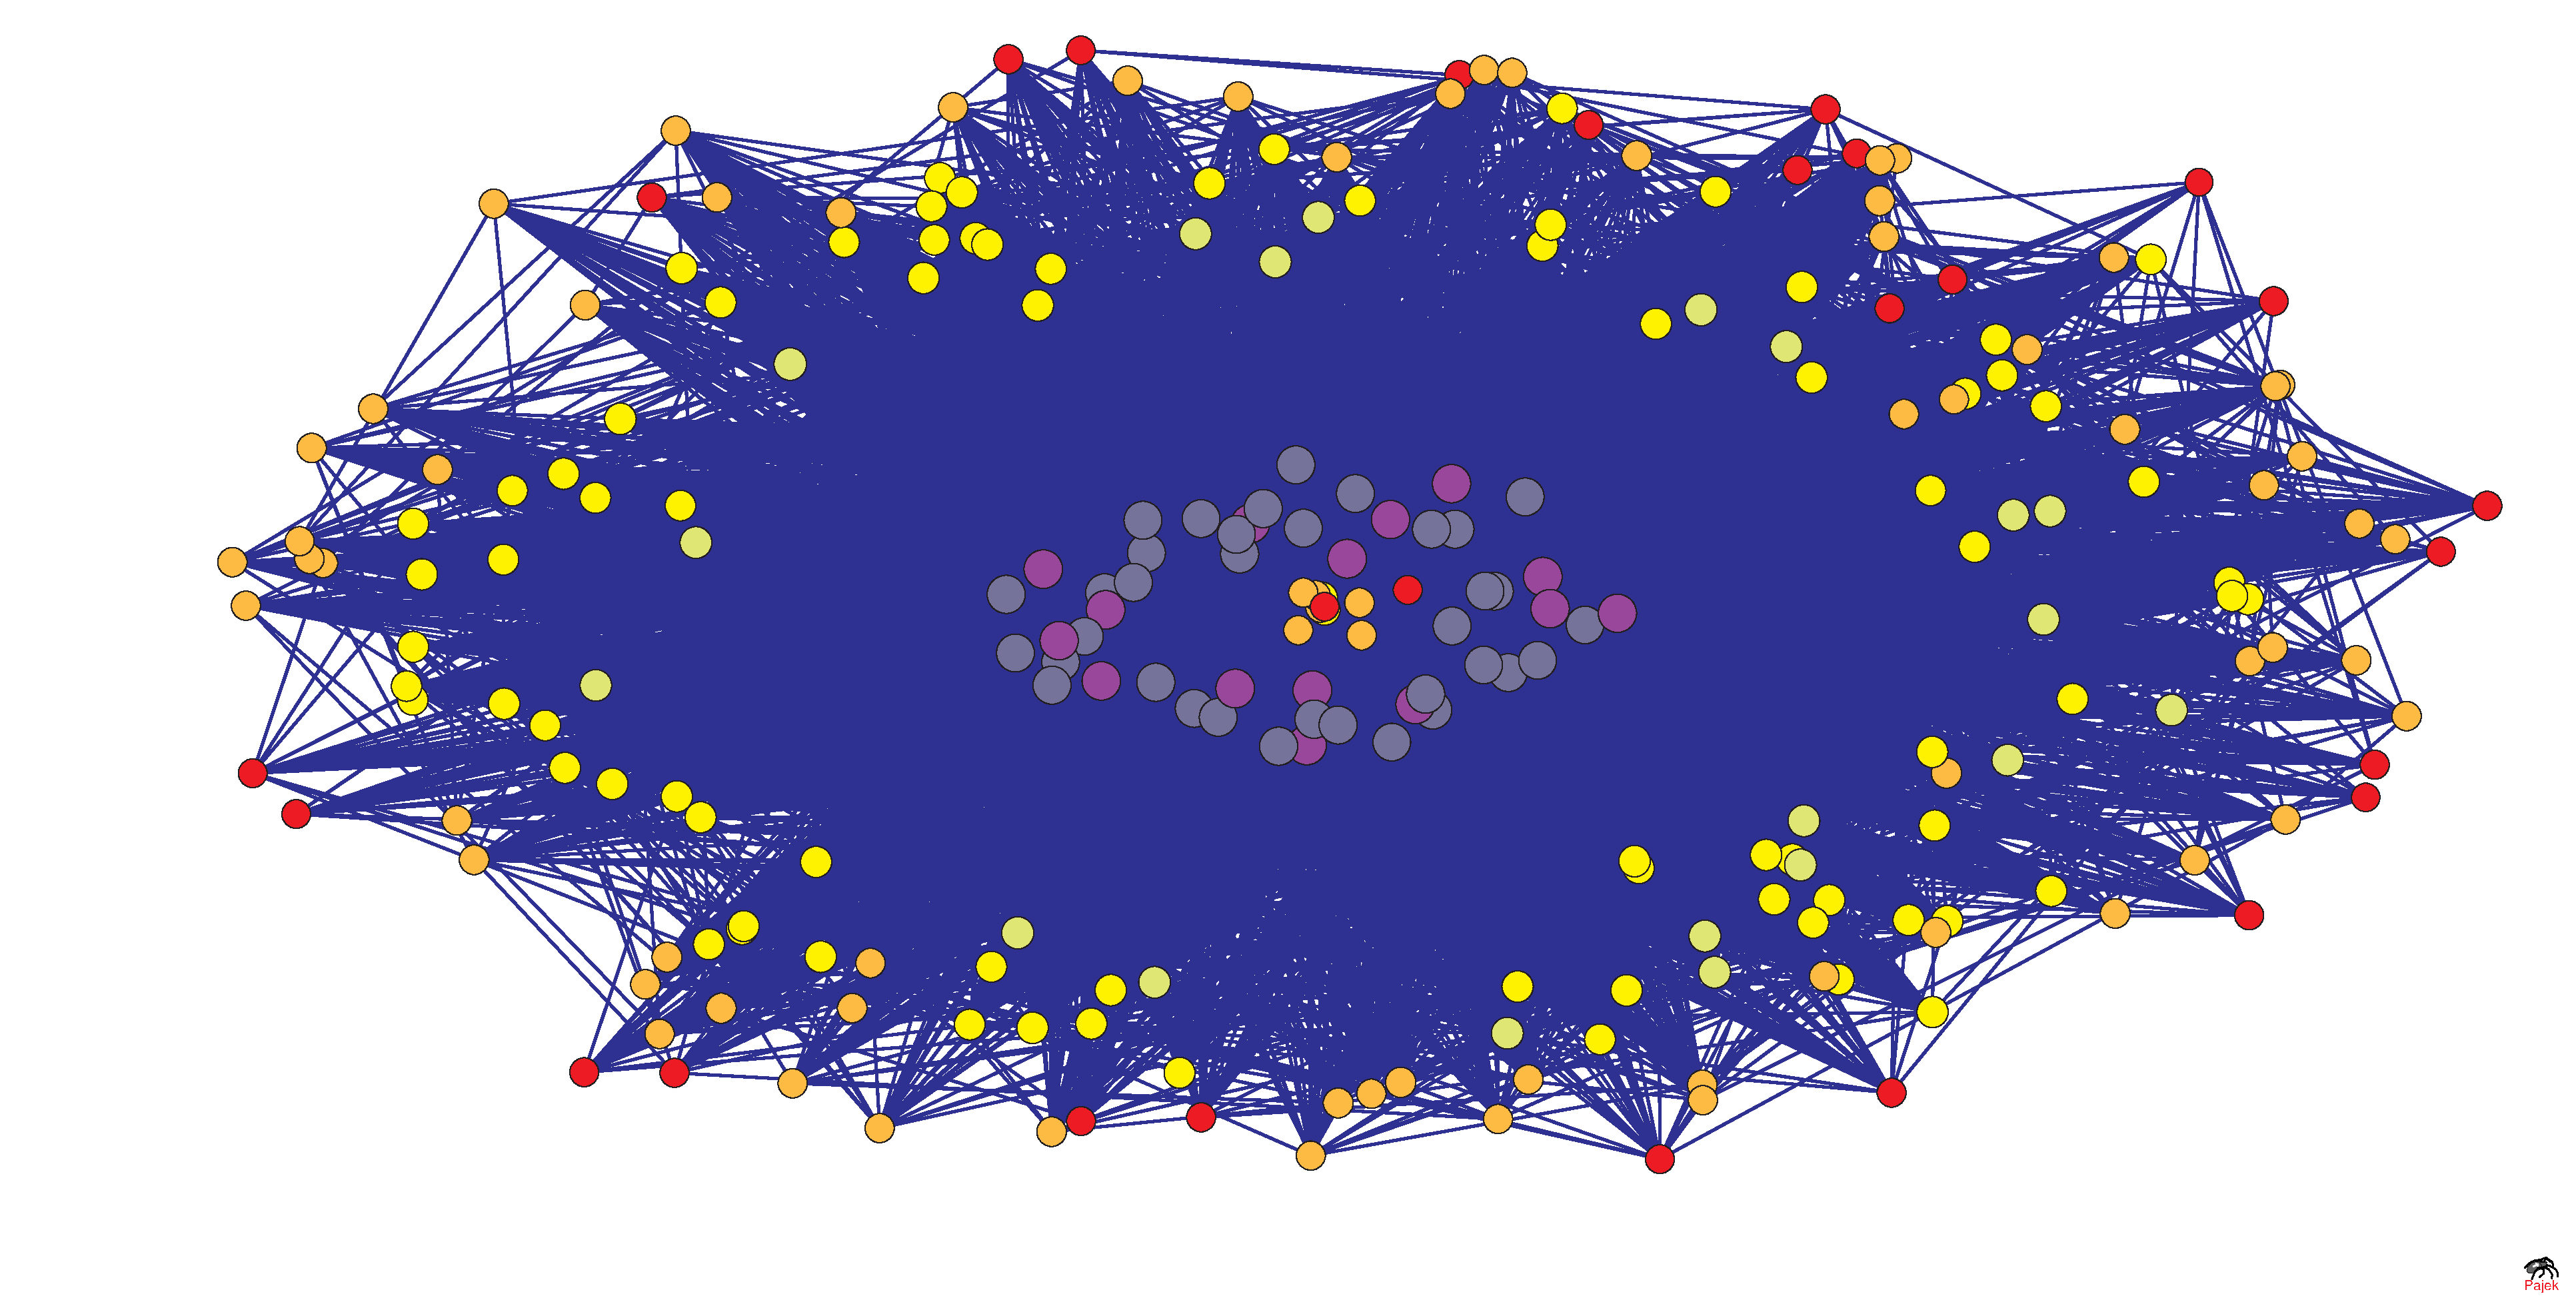
\includegraphics[width=0.45\textwidth]{toy2_k_centrality}
}
\caption{Centrality Measures of "Tripartite" Graph}
\label{fig:centrality2}
\end{figure}

\begin{figure}[h!]
\centering
\subfigure[Betweenness Centrality Partitioned into 2 Clusters]{
    \includegraphics[width=0.45\textwidth]{betw_kmeans}
}
\subfigure[Closeness Centrality Partitioned into 2 Clusters]{
    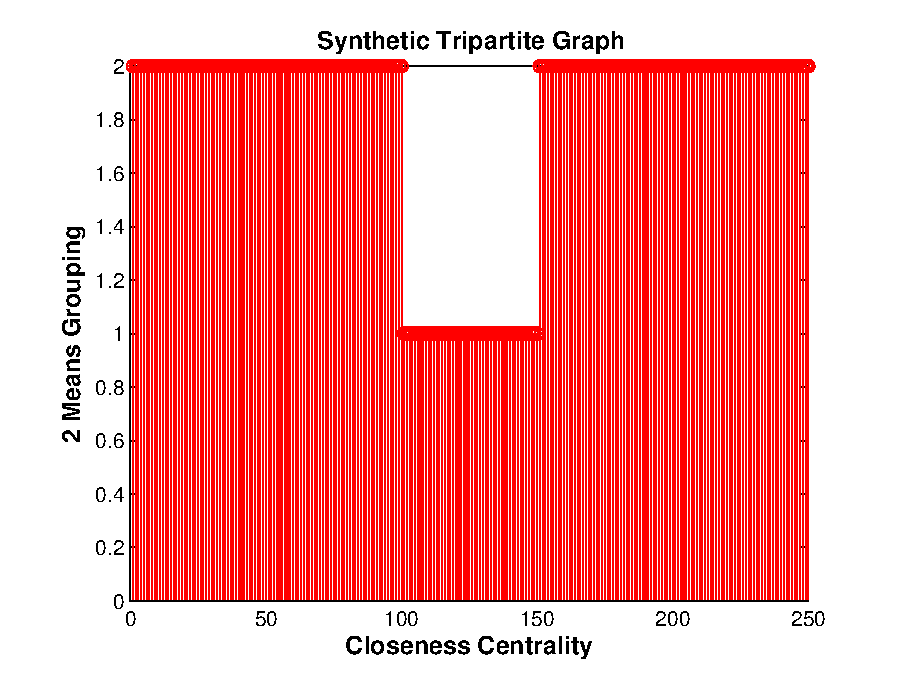
\includegraphics[width=0.45\textwidth]{close_kmeans}
}
\subfigure[Current-Flow Betweenness Centrality Partitioned into 2 Clusters]{
    \includegraphics[width=0.45\textwidth]{cfbetw_kmeans}
}
\subfigure[Current-Flow Closeness Centrality Partitioned into 2 Clusters]{
    \includegraphics[width=0.45\textwidth]{cfclose_kmeans}
}
\subfigure[$k$-Means Centrality Partitioned into 2 Clusters]{
    \includegraphics[width=0.45\textwidth]{kcent_kmeans}
}
\caption{Cluster Recovery Test on "Tripartite" Graph}
\label{fig:test1}
\end{figure}


Our next test is the average distance test, where we sort the vector of centrality values in descending order. In the sorted vector, we expect that the first 50 nodes to correspond to the nodes of the inner cluster and the last 200 nodes to correspond to nodes of the outer clusters of the "tripartite" graph because of their expected centrality values. For every cut point $p$, which is an index of the vector that divides it into two groups, we the compute average pairwise distances $\sigma_1$ and $\sigma_2$ of the two groups. Then we plot $\lambda = \frac{\sigma_1 + \sigma_2}{2}$ for each cut point $p$. We expect that the minimum value of $\lambda$ to be at $p=50$ since that is where the vector is divided into two groups of high centrality values and low centrality values, that is the inner cluster and the outer clusters, respectively. As a result, the difference in centrality values within each group should be small as compared to other instances for different value $p$. The test is explained in more details as follows:
\begin{enumerate}
\item Divide the vector of centrality values into two groups by the index $p$, so their sizes are $p$ and $q$ such that $p+q=n$.
\item Compute the distance matrices $D_1$ and $D_2$ based on Euclidean norm for both groups and compute the average pairwise distances $\sigma_1$ and $\sigma2$ where
\begin{align}
  \sigma_1 = \frac{\sum_{k=1}^p [D_1 \cdot \mathds{1}]_k}{\binom{p}{2}} \quad \quad
      \sigma_2 = \frac{\sum_{k=1}^q [D_2 \cdot \mathds{1}]_k}{\binom{q}{2}}
\end{align}
where $\mathds{1}$ is the ones vector.
\item Compute $\lambda = \frac{\sigma_1+\sigma_2}{2}$ and plot it with its corresponding cut point $p$. 
\end{enumerate}
The plots of the test are displayed in Figure \ref{fig:test2}.

\begin{figure}[h!!!]
\centering
\subfigure[Average Distance for Betweenness Centrality]{
    \includegraphics[width=0.45\textwidth]{avgdist_betw}
}
\subfigure[Average Distance for Closeness Centrality]{
    \includegraphics[width=0.45\textwidth]{avgdist_close}
}
\subfigure[Average Distance for Current-Flow Betweenness]{
    \includegraphics[width=0.45\textwidth]{avgdist_cfbetw}
}
\subfigure[Average Distance for Current-Flow Closeness]{
    \includegraphics[width=0.45\textwidth]{avgdist_cfclose}
}
\subfigure[Average Distance for $k$-Means Centrality]{
    \includegraphics[width=0.45\textwidth]{avgdist_kcent}
}
\caption{Average Distance Test on "Tripartite" Graph}
\label{fig:test2}
\end{figure}

The results show that closeness centrality, current-flow betweenness, and $k$-means centrality performed well in this test since $\lambda$ obtain its minimum at $p=50$. Because there are edges between the outer clusters of the "tripartite" graph, $\lambda$ for current-flow closeness does not obtain its minimum at $p=50$. Furthermore, $\lambda$ for betweenness centrality is unable to obtain its minimum $p = 50$ because it does not account for the information spread on non-shortest paths.

\subsection{Florentine Network}
Now we compute the centrality measures on the Florentine network, consisting of the fifteen most influential families of 15th century Florentine, Italy. Because the Medici family was considered the most influential at the time, its centrality values is expected to be high for any centrality measure. The results of the centrality measures are shown in Figure \ref{fig:florentine}.

From our results, we see that the purple node with largest size in the graph is the Medici family for all centrality measures. However, for betweenness centrality and $k$-means centrality, the other nodes do not have much influence on the graph as evident by their sizes. On the other hand, the other centrality measures show that the other nodes have some considerable influences.

\begin{figure}[h!!!]
\centering
\subfigure[Betweenness Centrality of Florentine Network]{
    \includegraphics[width=0.45\textwidth]{FlorentineBetweenness2}
}
\subfigure[Closeness Centrality of Florentine Network]{
    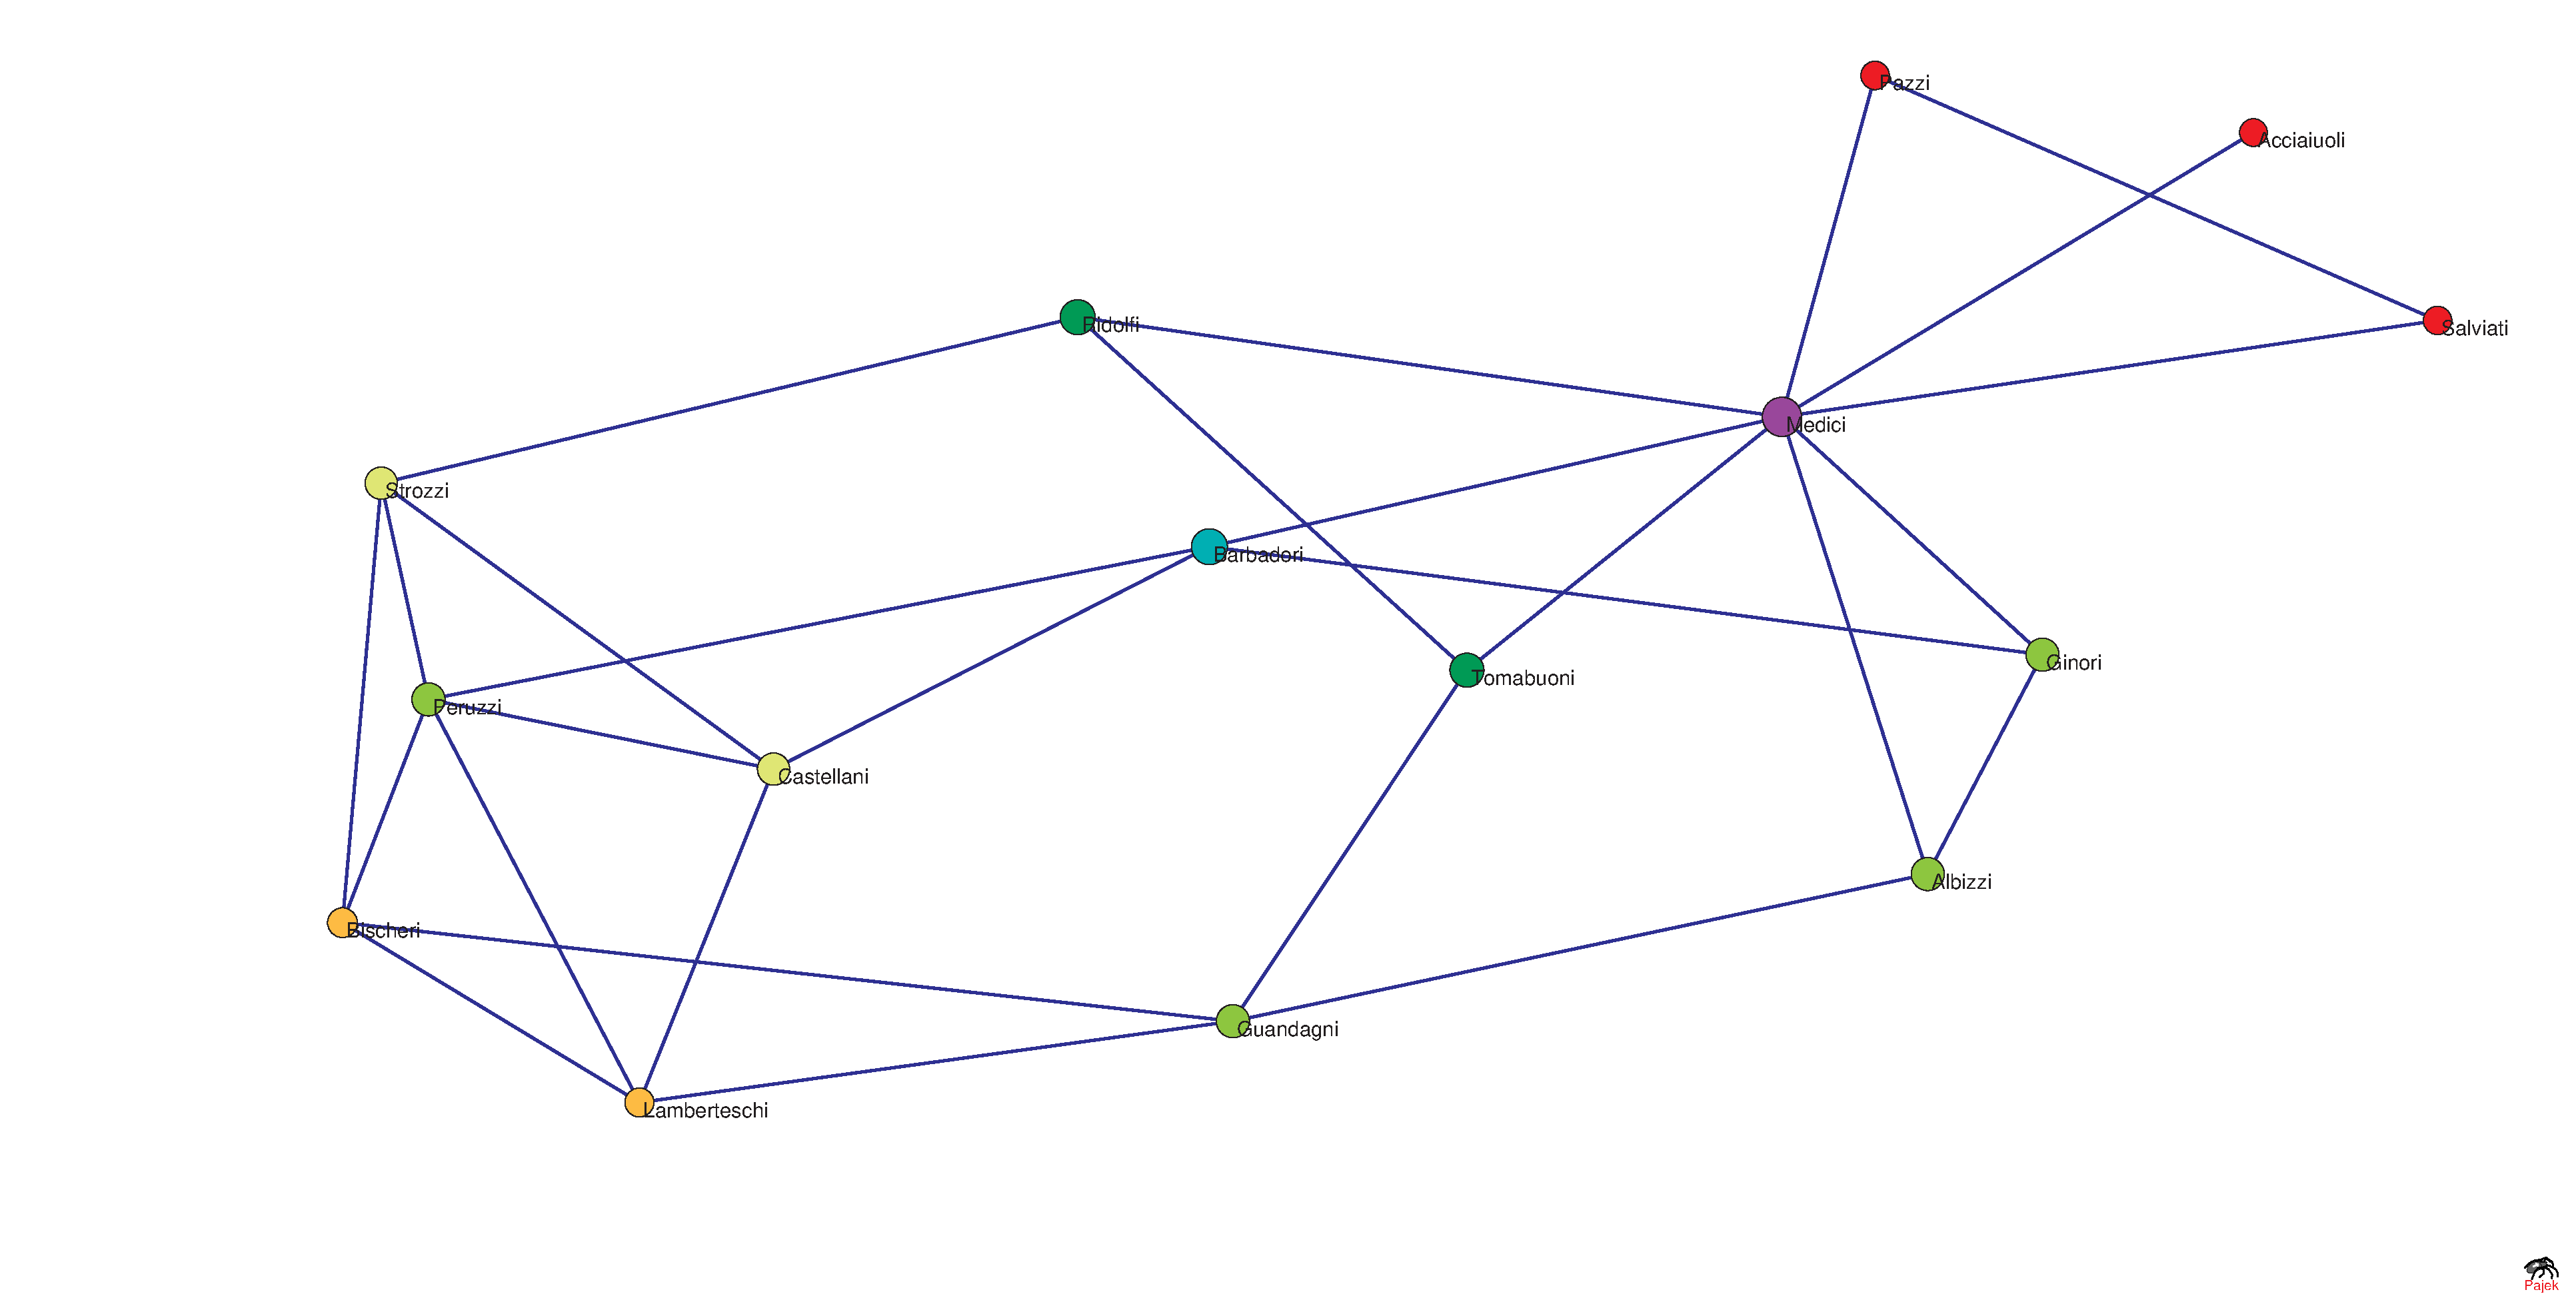
\includegraphics[width=0.45\textwidth]{Florentine_closeness2}
}
\subfigure[Current-Flow Betweenness Centrality of Florentine Network]{
    \includegraphics[width=0.45\textwidth]{florentine_current_flow_betweenness2}
}
\subfigure[Current-Flow Closeness Centrality of Florentine Network]{
    \includegraphics[width=0.45\textwidth]{florentine_current_flow_closeness2}
}
\subfigure[$k$-Means Centrality of Florentine Network]{
    \includegraphics[width=0.45\textwidth]{FlorentineKcentrality2}
}
\caption{Centrality Measures on Florentine Network}
\label{fig:florentine}
\end{figure}

\subsection{Reed College's Social Network}
For a larger real data set, we compute the centrality measures on the Facebook friends network of Reed College containing 962 nodes. The results are shown in Figure \ref{fig:reed}

\begin{figure}[h!!!]
\centering
\subfigure[Betweenness Centrality of Reed Network]{
    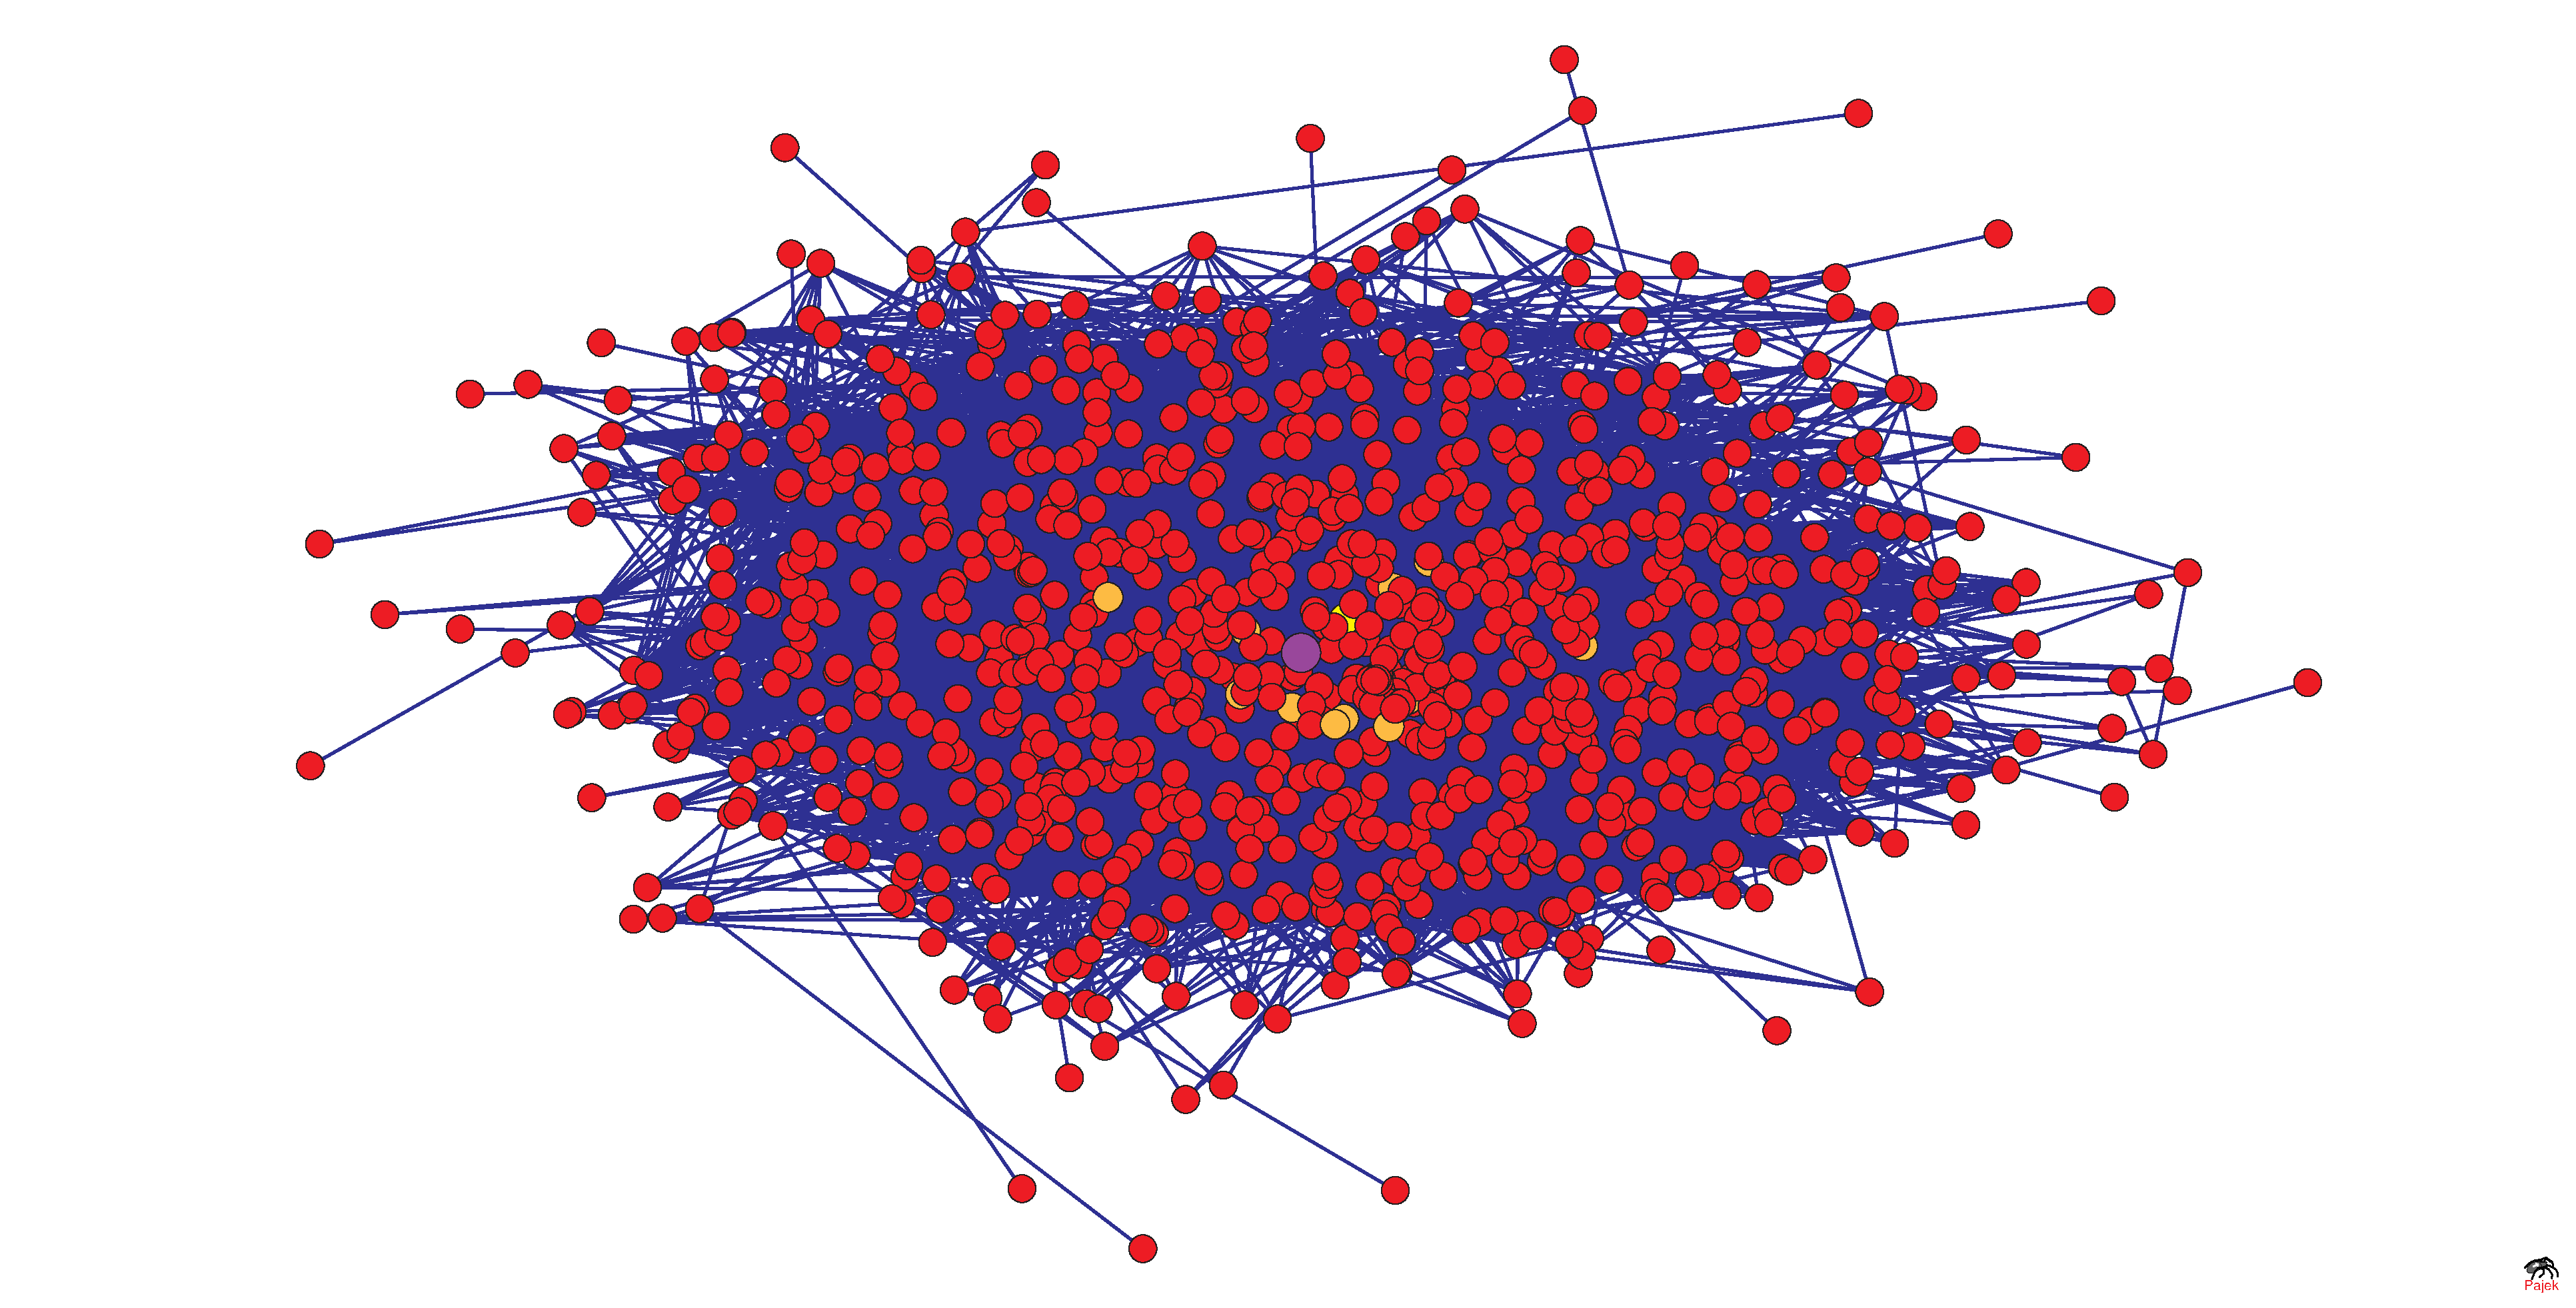
\includegraphics[width=0.45\textwidth]{reed_betweenness}
}
\subfigure[Closeness Centrality of Reed Network]{
    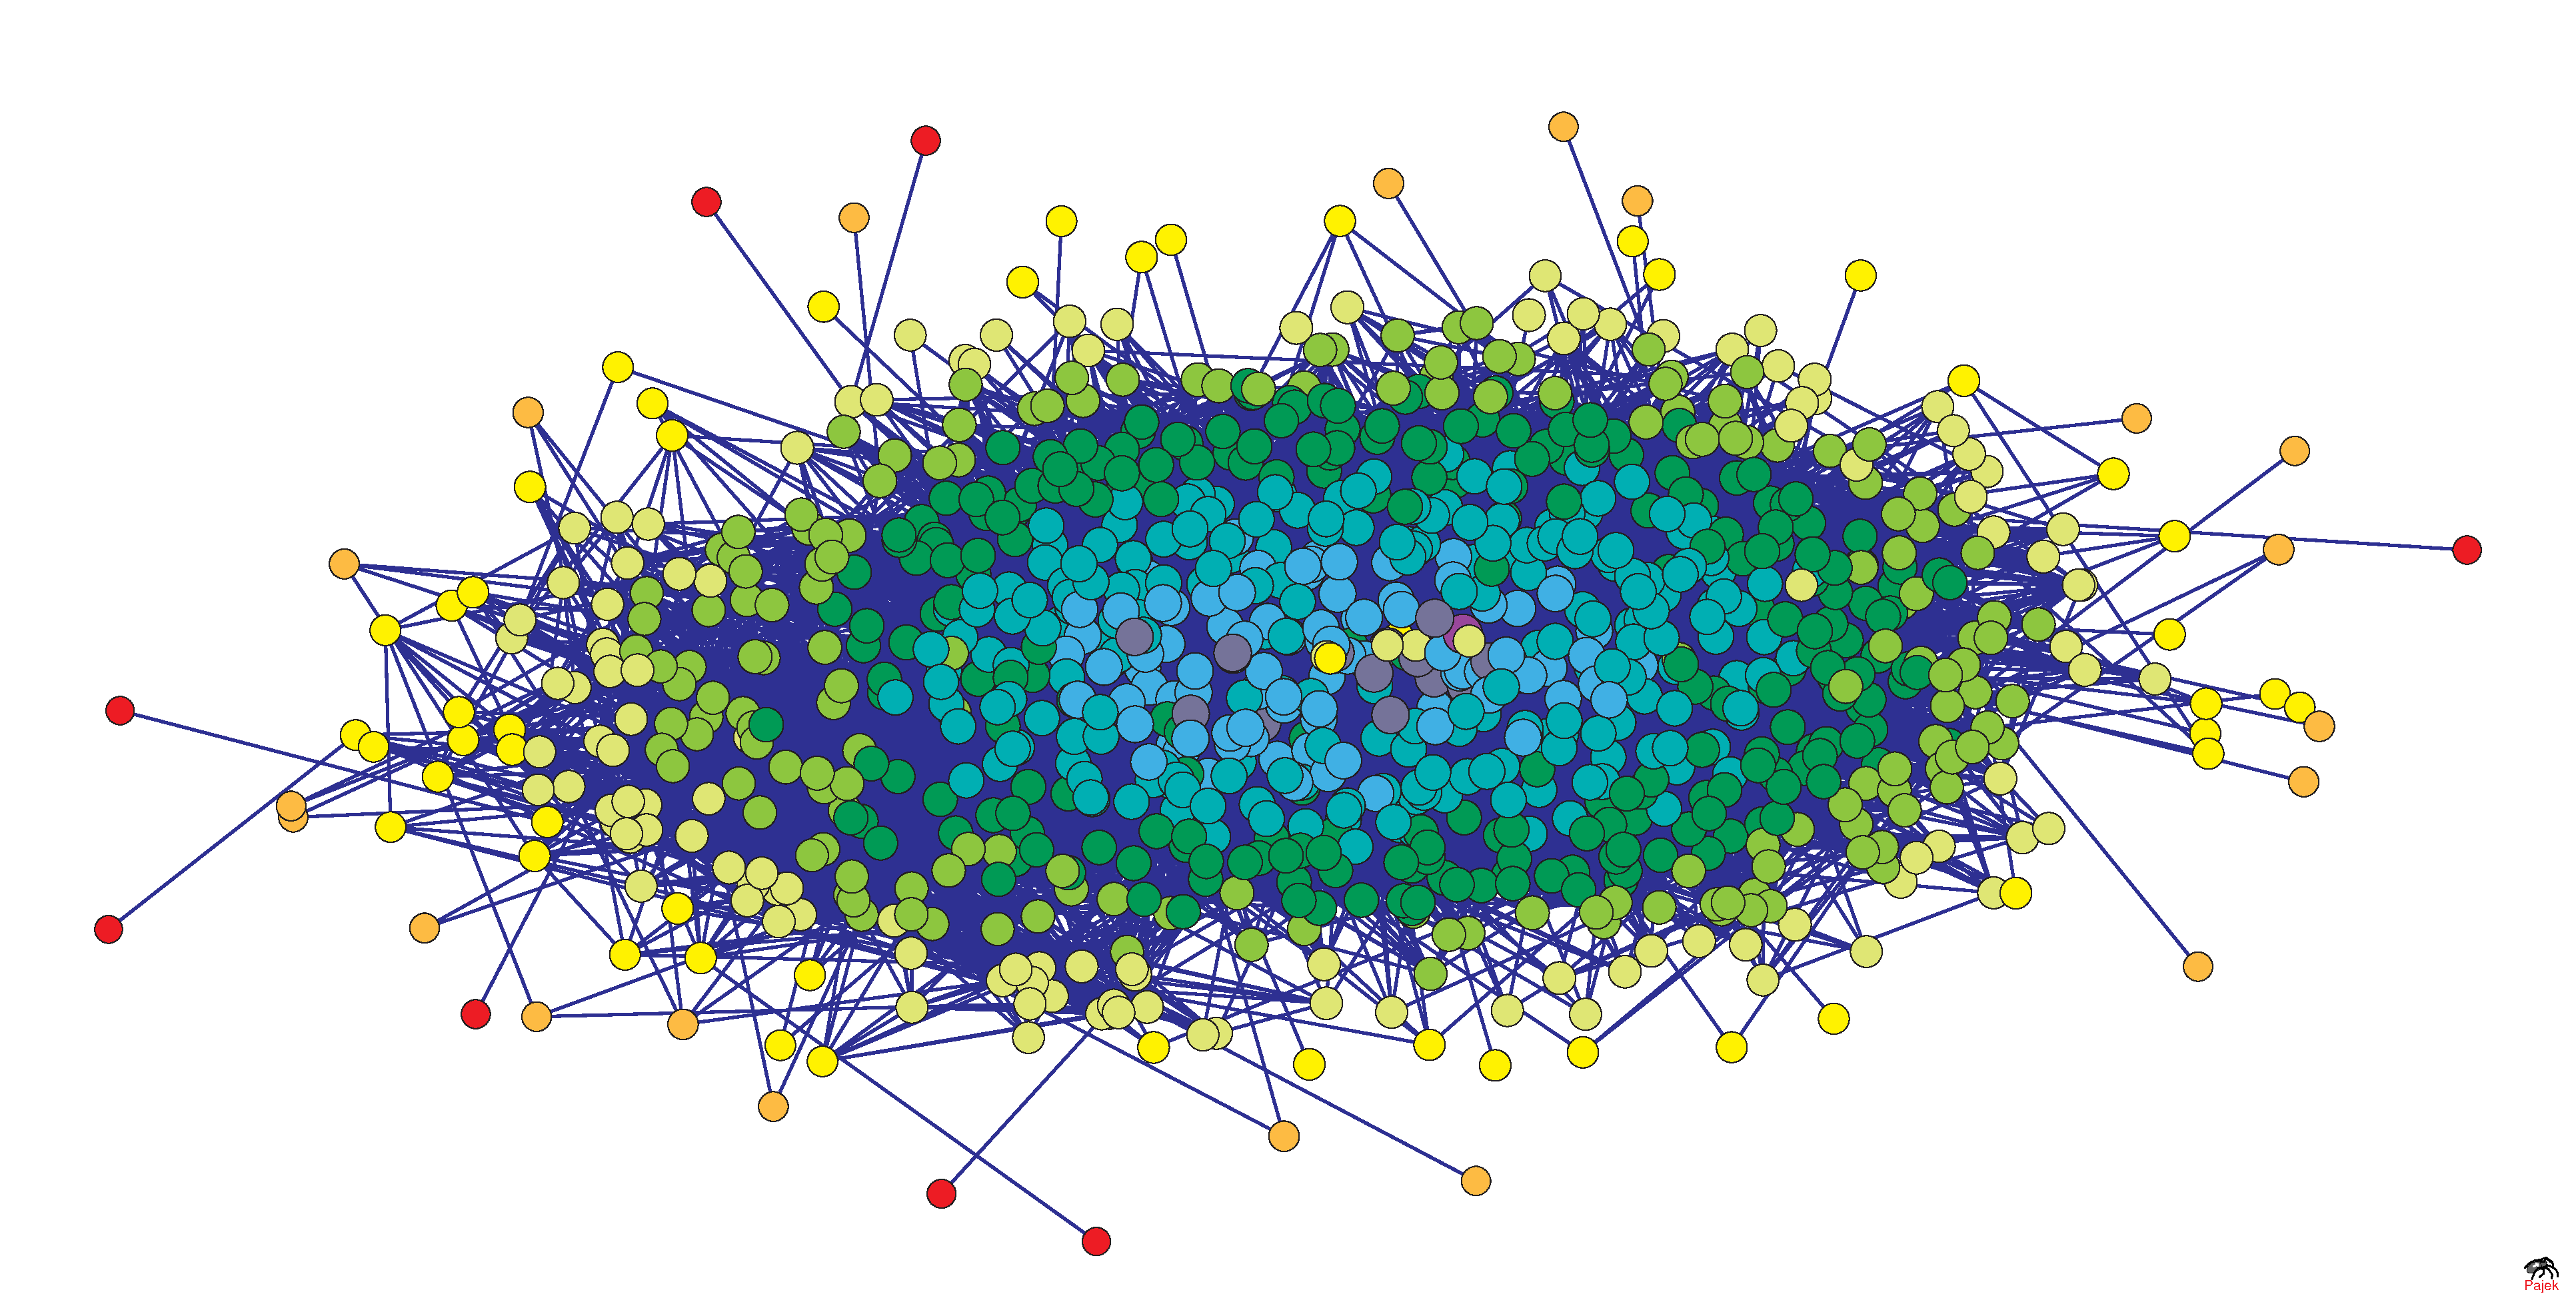
\includegraphics[width=0.45\textwidth]{reed_closeness}
}
\subfigure[Current-Flow Betweenness Centrality of Reed Network]{
    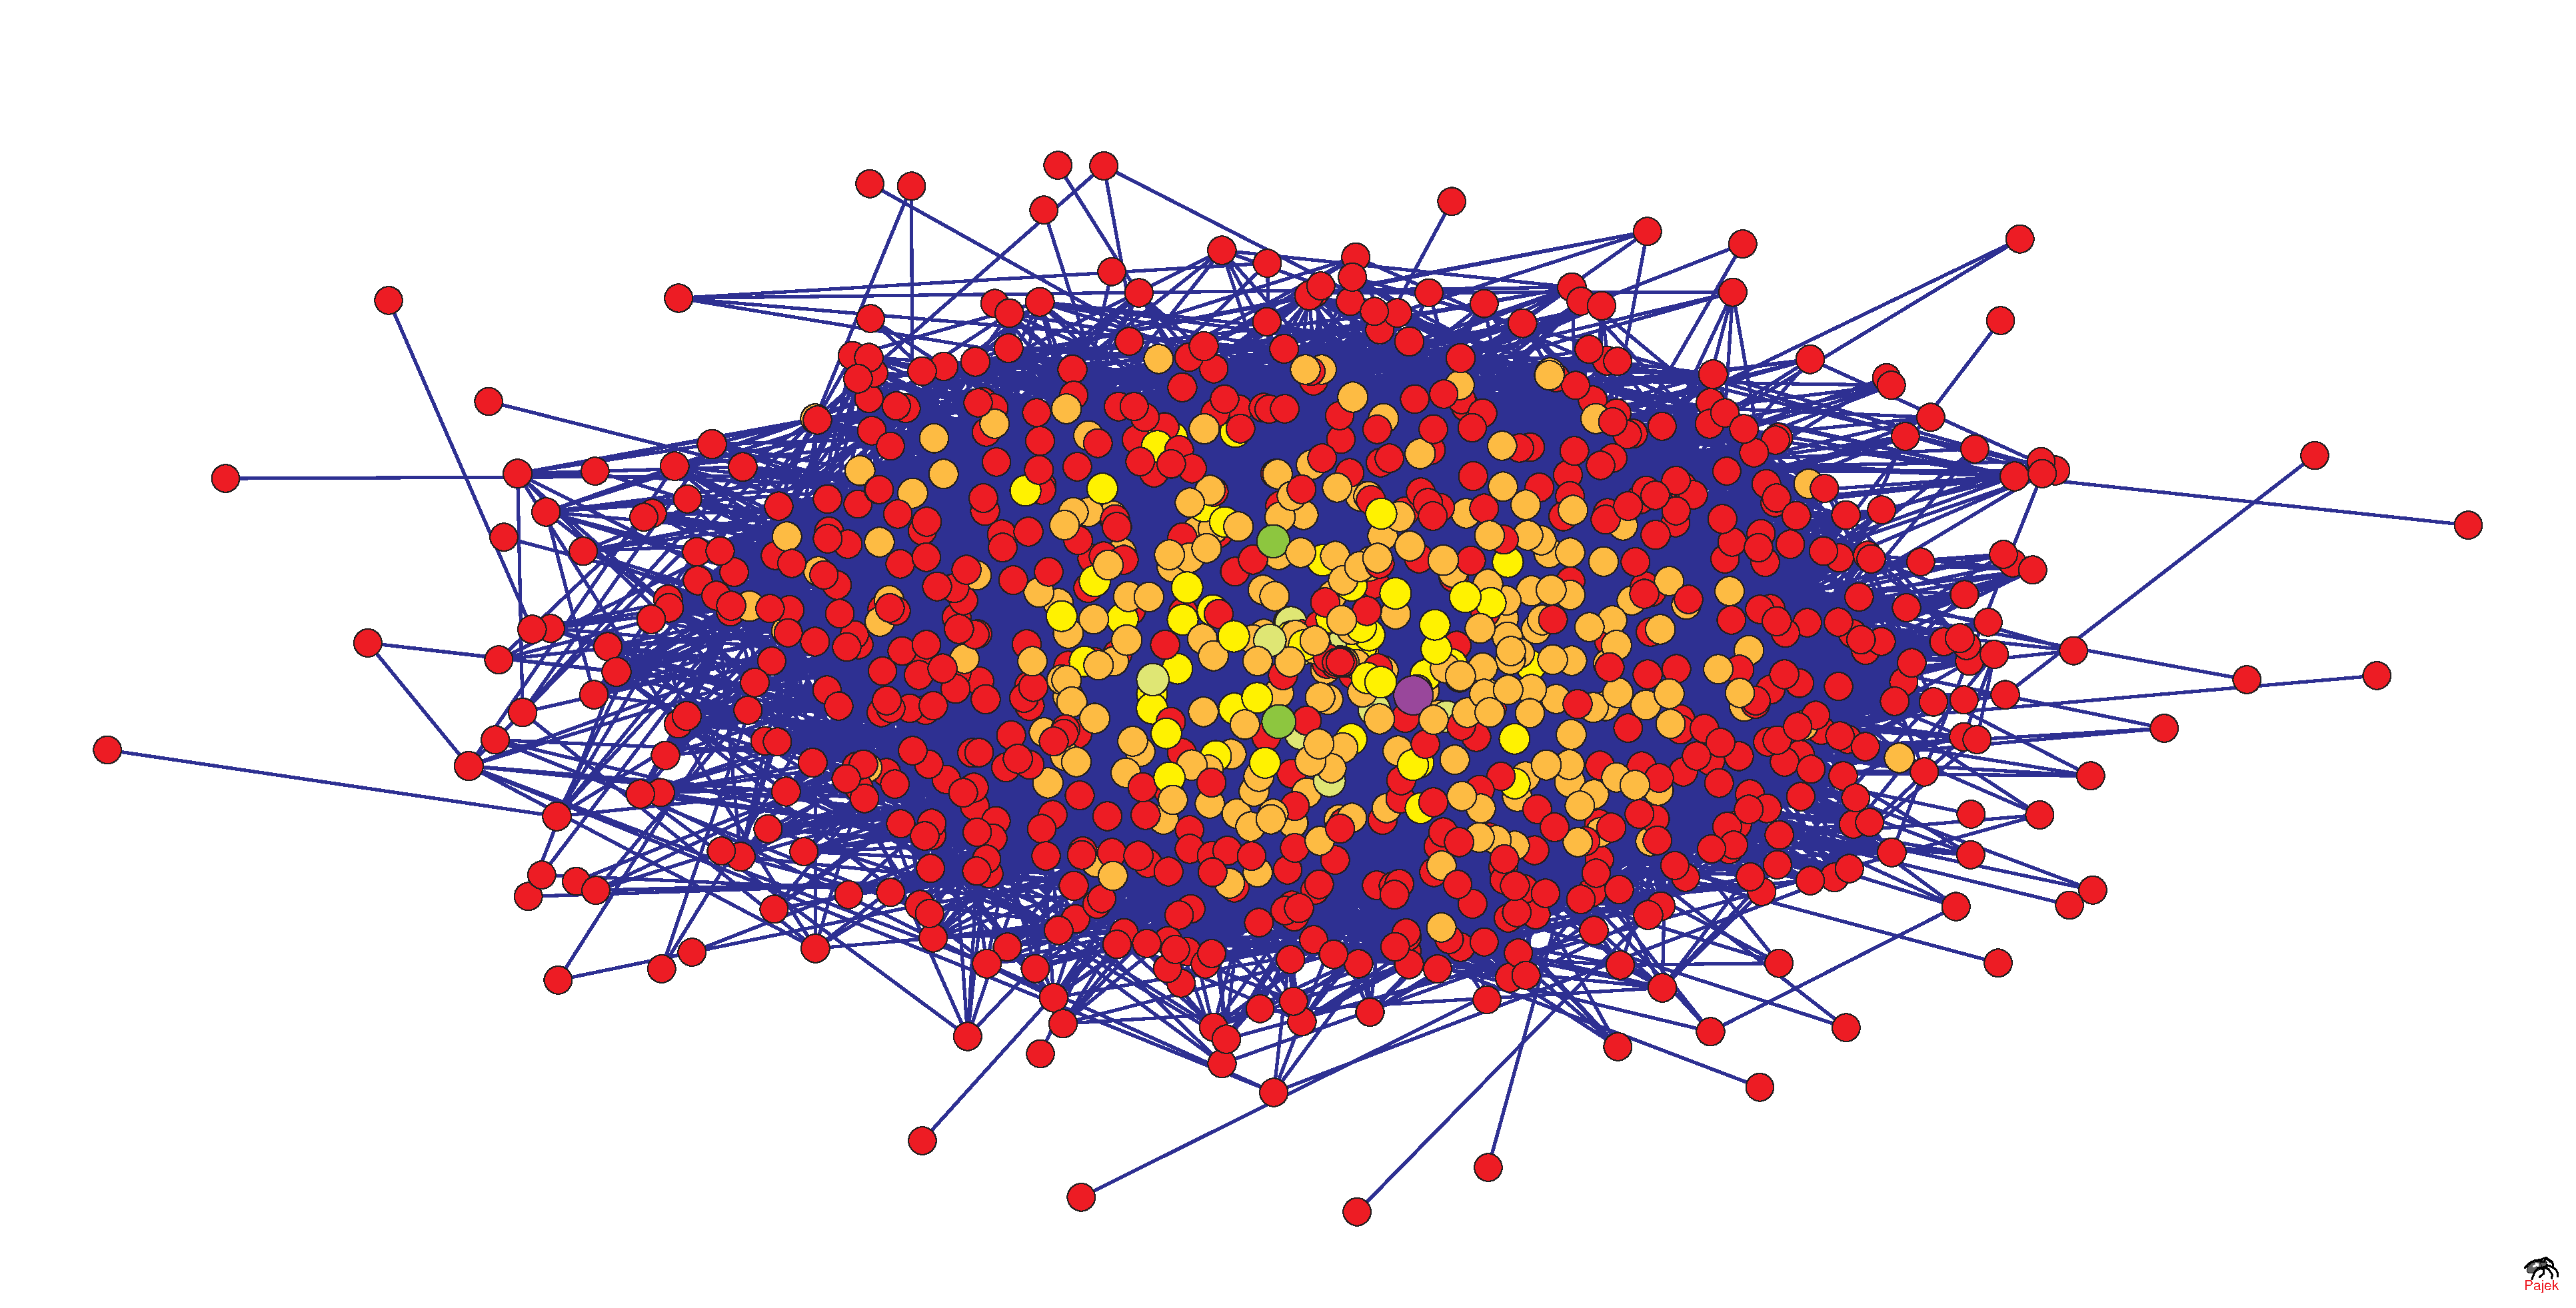
\includegraphics[width=0.45\textwidth]{reed_current_flow_betweenness}
}
\subfigure[Current-Flow Closeness Centrality of Reed Network]{
    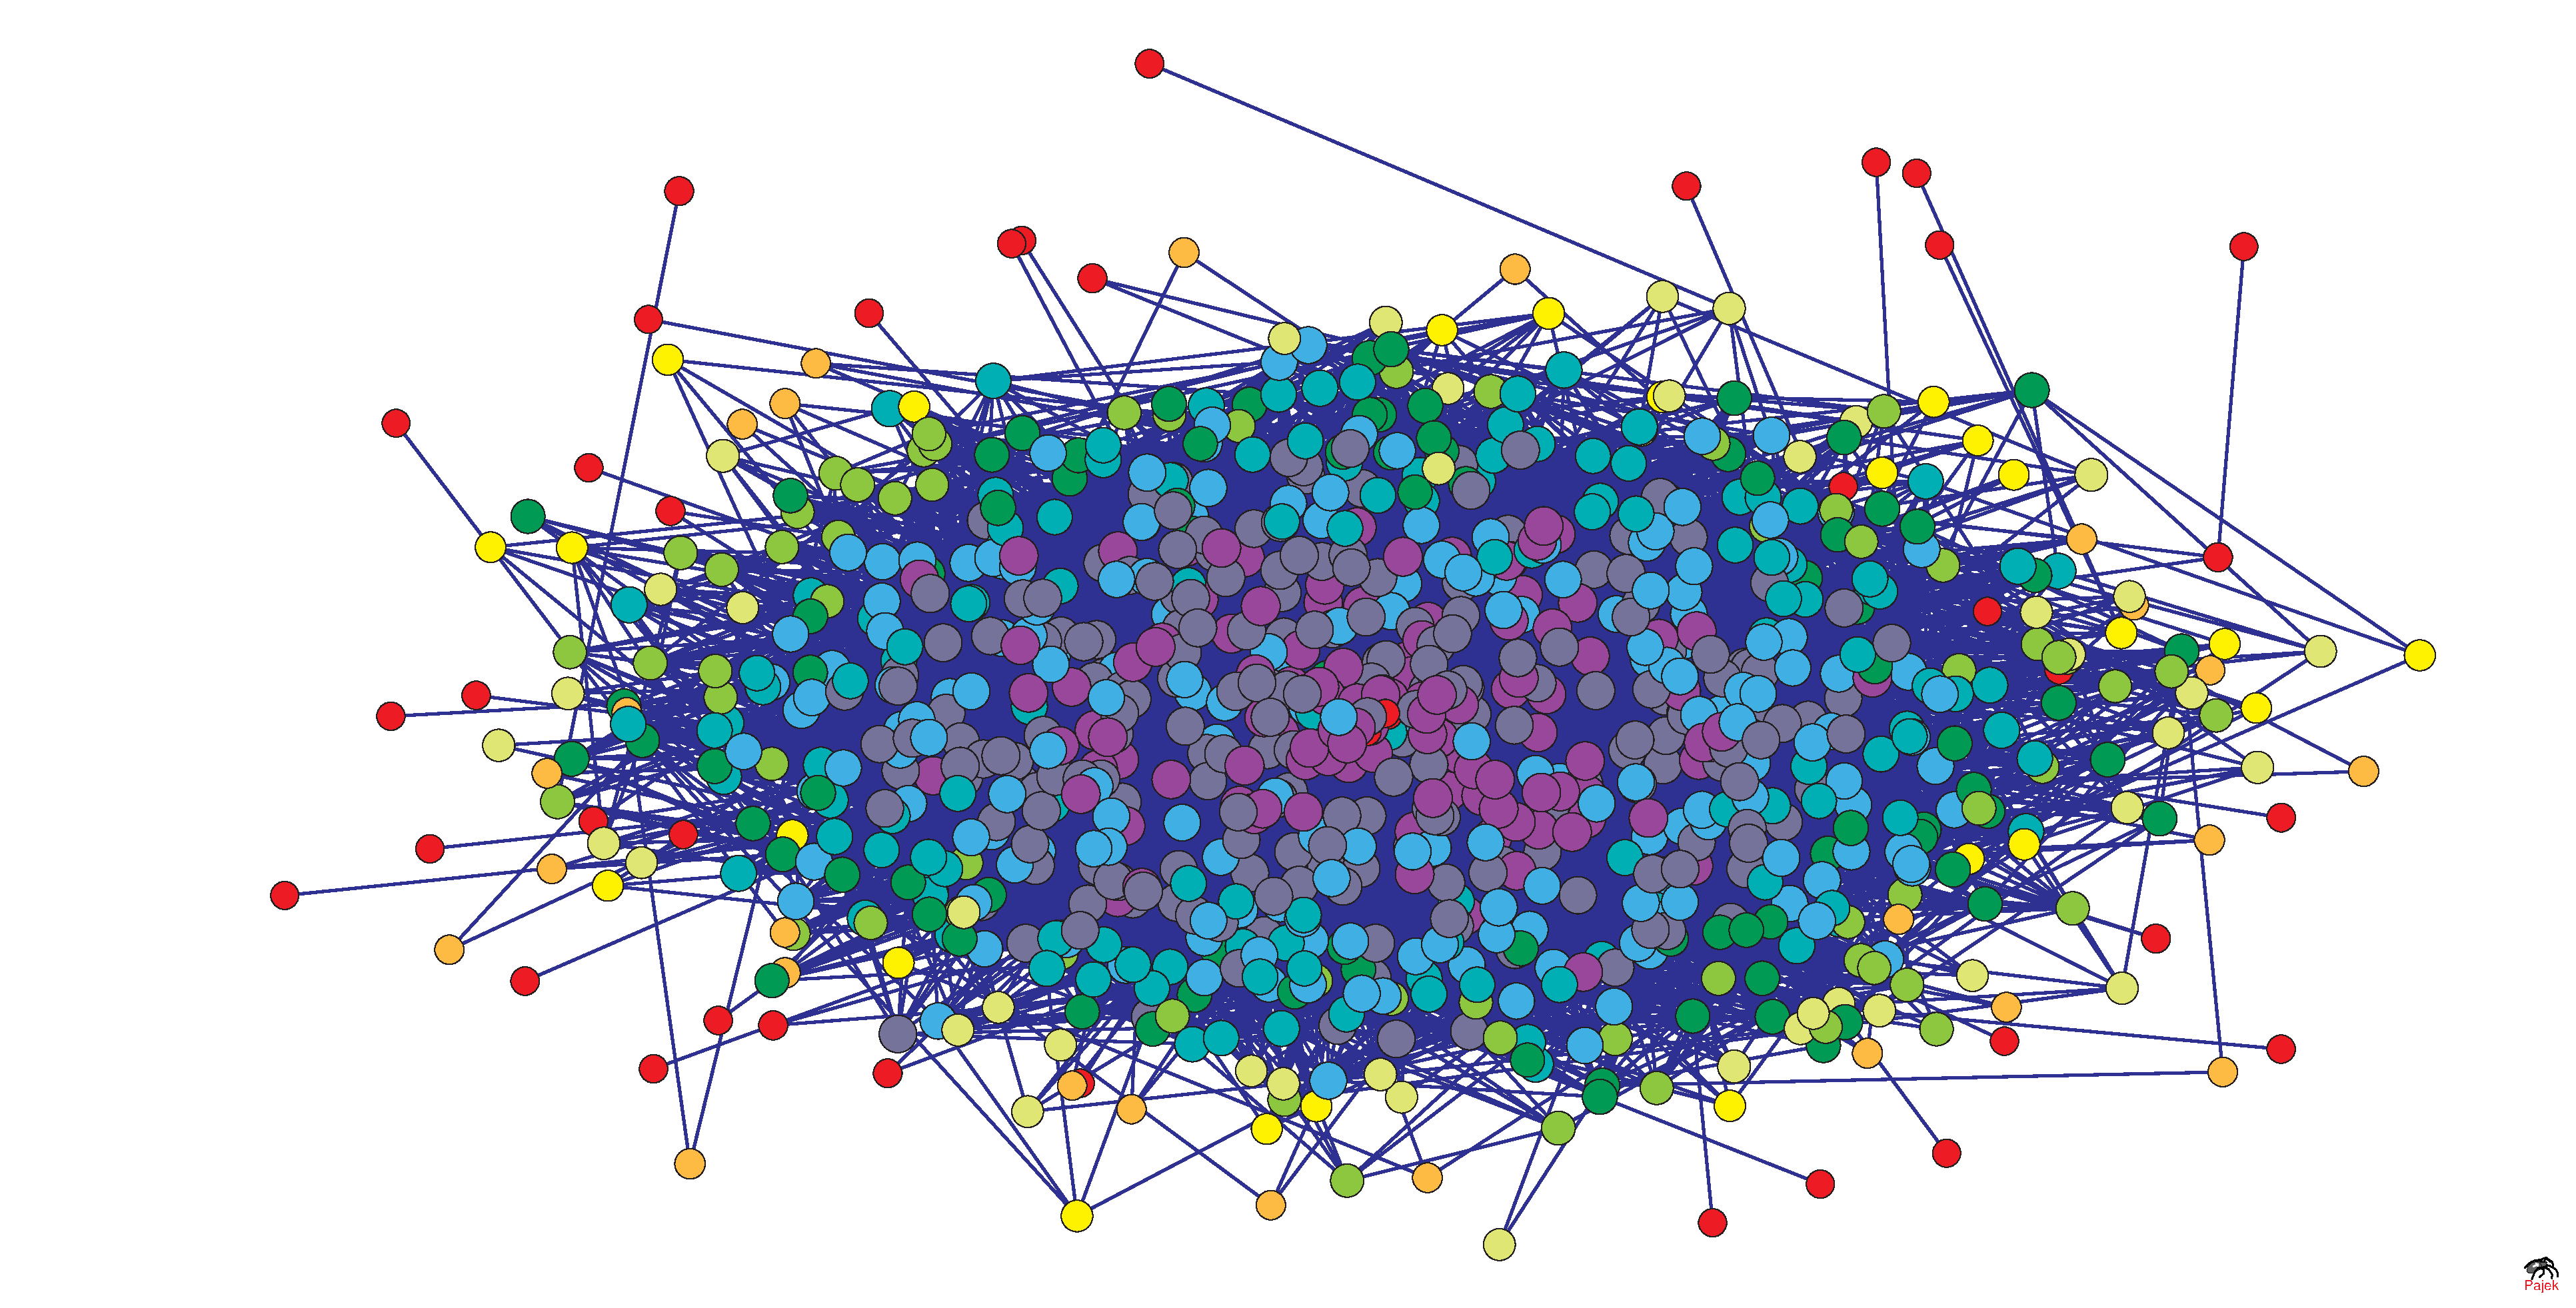
\includegraphics[width=0.45\textwidth]{reed_current_flow_closeness}
}
\subfigure[$k$-Means Centrality of Reed Network]{
    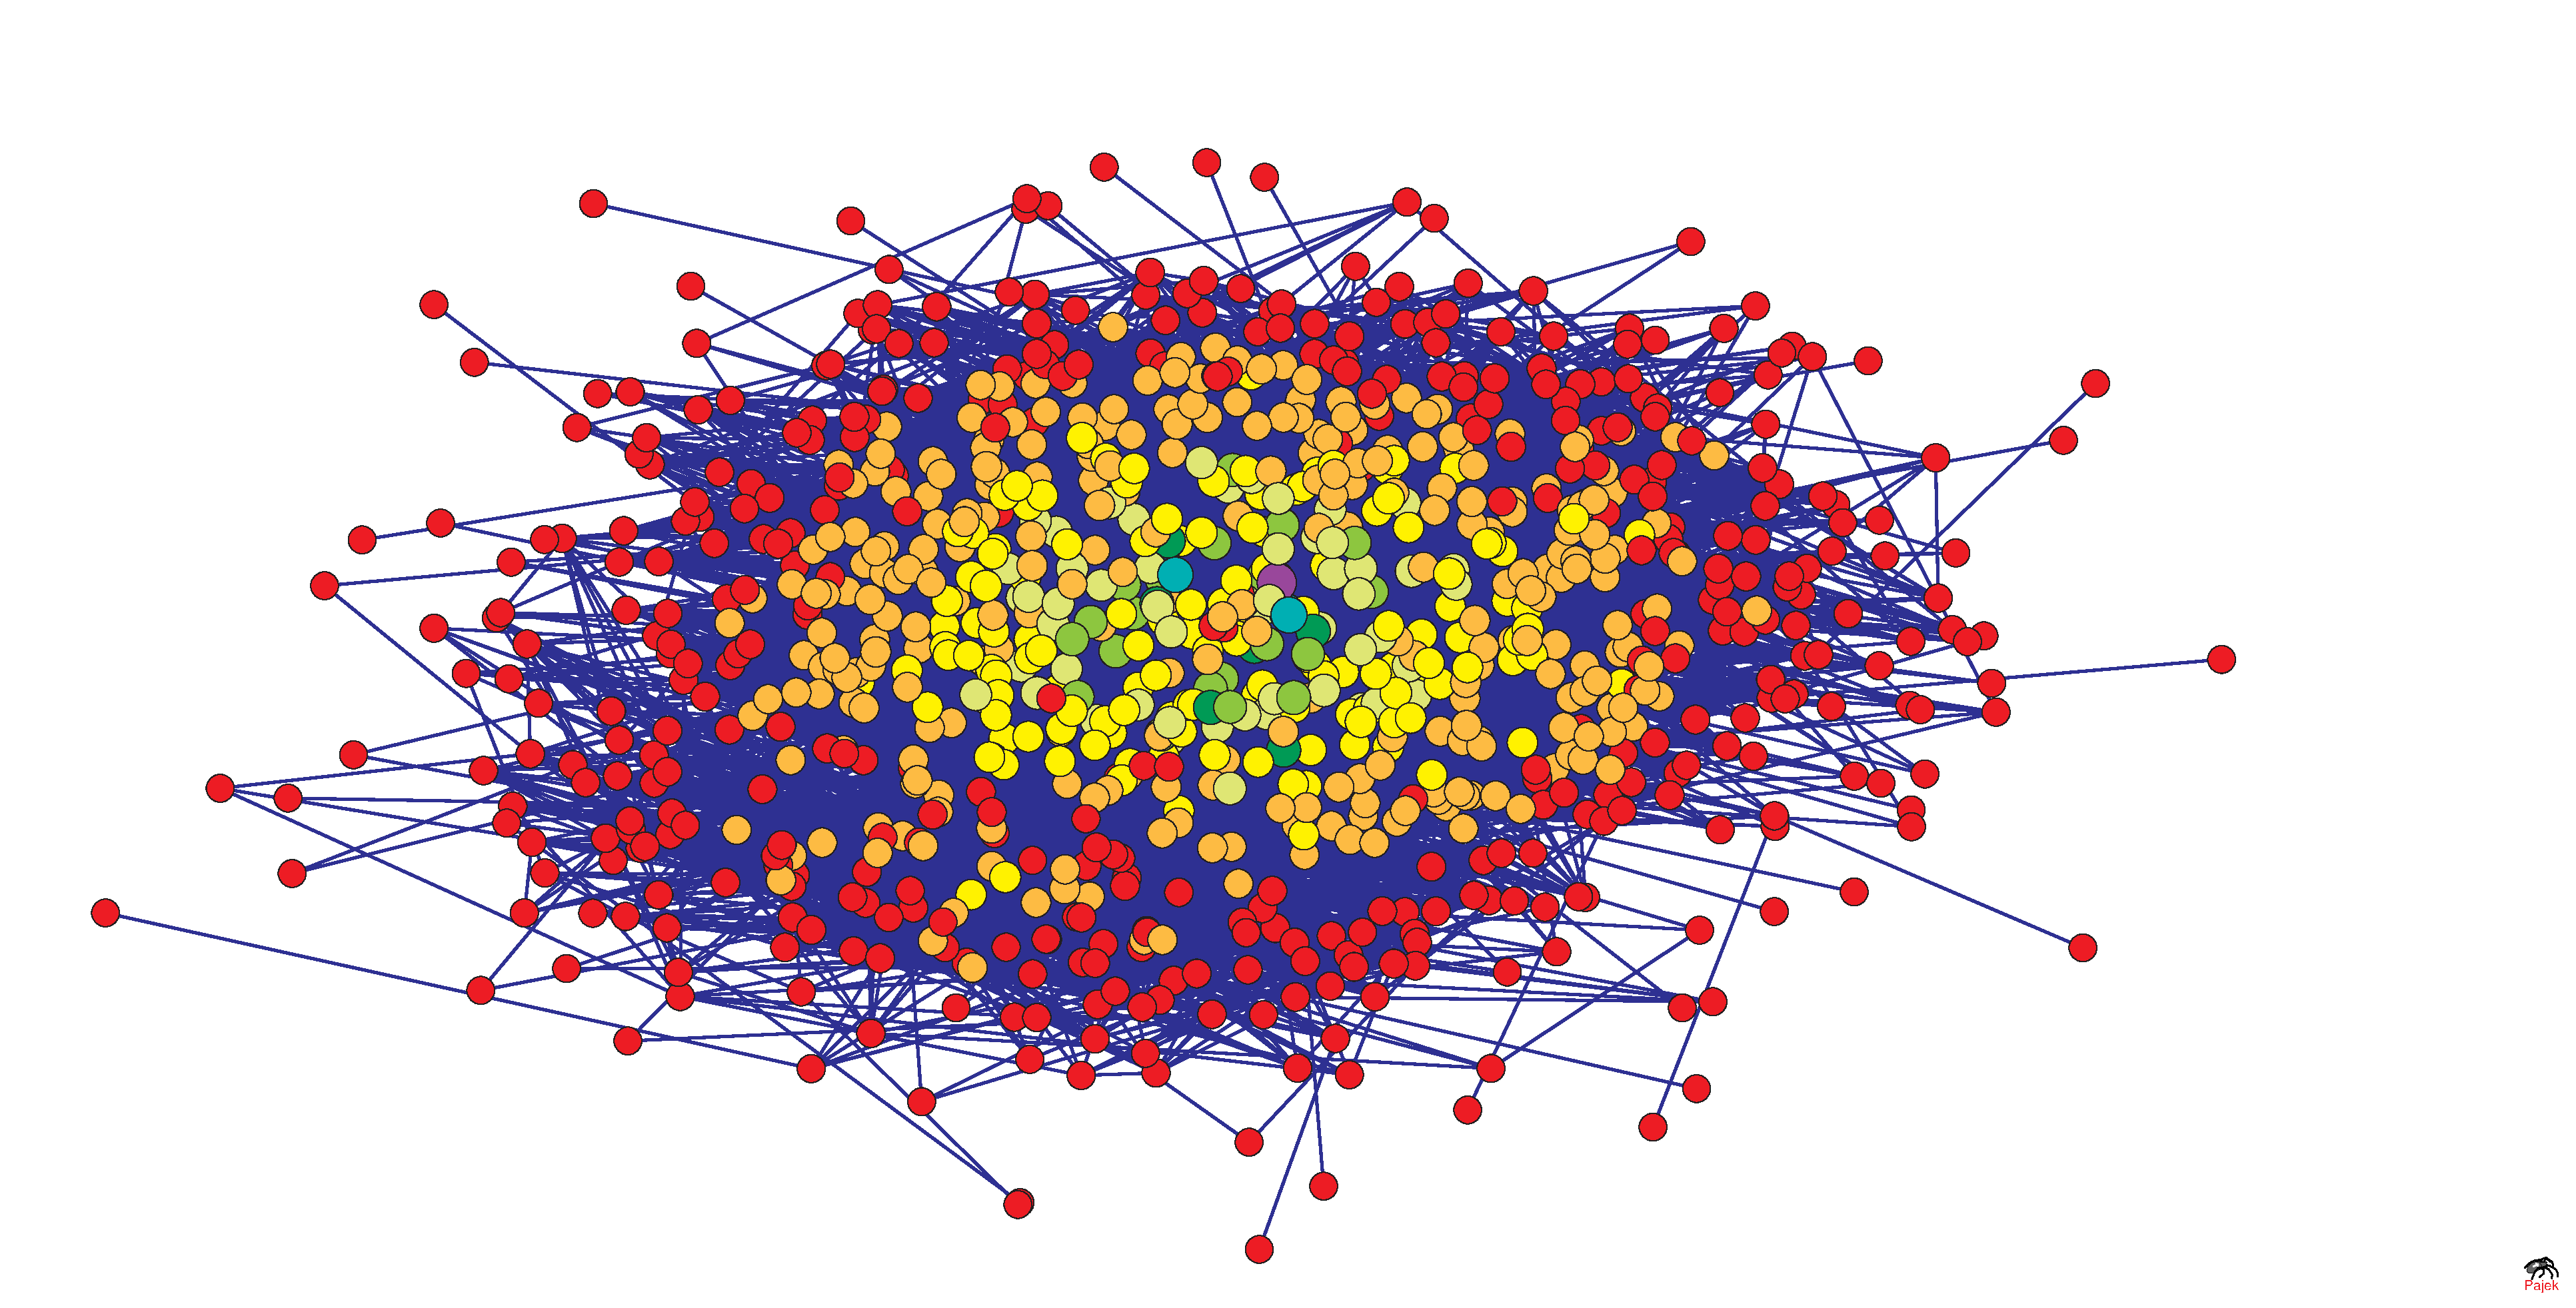
\includegraphics[width=0.45\textwidth]{reed_k_centrality}
}
\caption{Centrality Measures on Reed Network}
\label{fig:reed}
\end{figure}

Similarly to the "tripartite" graph, we observe that betweenness centrality performs poorly since majority of the nodes have low centrality values. The other four centrality measures have varying degrees of success of distinguishing the nodes. Closeness and current-flow closeness centrality have very few nodes of low centrality values and more nodes of intermediate centrality values. Current-flow betweenness and $k$-means centrality have similar results, but current-flow betweenness has more nodes with low centrality values.  



\subsection{Discriminative Measure}
A centrality measure is considered useful if it is able to discriminate different node properties in a graph. In other words, it is able to detect nodes with considerable, but not high or low, amount of influences. To determine how well a centrality measure discriminates the nodes, we compute the discrimination measure. To obtain the discrimination measure $\delta$, we compute the distance matrix $D$ based on the Euclidean norm from the vector of centrality values so that we have
\begin{align}
 	\delta=\sum_{i=1}^n \left[\frac{v}{\parallel v\parallel}\right]_i   \qquad \textrm{where} \quad v = \frac {D*\mathds{1}}{n}
\end{align}
In short, the discriminative measure is the sum of the normalized vector of averaged pairwise distances. Thus, a larger discrimination measure indicates that the centrality measure better distinguishes different node properties. We compute the discriminative measure of the centrality measures for both Florentine network and Reed network and their results are shown in Figure \ref{fig:discriminative}

\begin{figure}[h!!!]
\centering
\subfigure[Discriminative Measures of Florentine Network]{
    \includegraphics[width=0.45\textwidth]{discriminative_Florentine}
}
\subfigure[Discriminative Measures of Reed Network]{
    \includegraphics[width=0.45\textwidth]{discriminative_Reed}
}
\caption{Discriminative Measures of Centrality Measures on Real Networks}
\label{fig:discriminative}
\end{figure}
 
From the results, the ranking of the centrality measures from least discriminative to most discriminative is as follows for both networks: betweenness, current-flow betweenness, $k$-means centrality, current-flow closeness, and closeness centrality.  This shows that the discrimination measure is consistent across networks. In the graphs, $k$-means centrality ranks in the middle, so it measures less discriminatively than closeness and current-flow closeness centrality but more discriminatively than betweenness and current-flow betweenness centrality. Furthermore, the discriminative measure for betweenness centrality verifies that it is not at all a useful centrality measure.

\subsection{Correlation with Node Degrees}
We compute the correlation between the values of the centrality measures and the node degrees. If the correlation with node degrees is high, this makes a centrality measure ineffective since computing the degrees would be more efficient for network analysis. The results are shown in Figure \ref{fig:correlation}. 

\begin{figure}[h!!!]
\centering
\subfigure[Correlation Between Centrality Measures and Node Degrees of Florentine Network]{
    \includegraphics[width=0.45\textwidth]{correlation_Florentine}
}
\subfigure[Correlation Between Centrality Measures and Node Degrees of Reed Network]{
    \includegraphics[width=0.45\textwidth]{correlation_Reed}
}
\caption{Correlation Between Centrality Measures and Node Degrees on Real Networks}
\label{fig:correlation}
\end{figure}

    Unlike the case of discriminative measure, we obtain different rankings from lowest to highest correlation between Florentine and Reed networks since a particular centrality measure's propensity to match node degree depends on the graph structure. For the Florentine network, the ranking are the following: closeness, betweenness, current-flow closeness, current-flow betweenness, and $k$-means centrality. For the Reed network, we have betweenness, current-flow closeness, closeness, current-flow betweeness, and $k$-means centrality. It is logical that $k$-means centrality would have a high correlation to node degree because it measures the tendency of a node to lie on a cut edge between two clusters of a network, where a cut node would be related to the number of edges adjacent to that node.

\section{Summary and conclusion}  \label{sec:conclusion}
%Summarize your work in this section.
After considering the results of the proposed $k$-means centrality on synthetic and real networks, we observe that it performs similarly to the existing centrality measures. $k$-means centrality can be utilized as a middle ground for the other centrality measures we compared it with. We also see that it is highly correlated to node degrees, which suggest that it might not be an effective centrality measure. However, as we mention in the introduction, a proper choice of centrality measure depends on the context for which it is being used. In our work, we focus mainly on the discriminative aspect of our new measure. It is certainly possible that the $k$-centrality would fare better under different circumstances. In particular, since this centrality is derived from the $k$-means algorithm, it may be fruitful to explore its results on other networks that have known distinct clusters within them.
\newpage
\bibliographystyle{siam}
\bibliography{project_math191}



\end{pagewiselinenumbers}

\end{document}



